\documentclass[12pt]{book}
\usepackage{multicol}
\usepackage{amsmath}
\usepackage{amsthm}
\usepackage{graphicx}
\usepackage{color}
\usepackage{bbm}
\usepackage[utf8]{inputenc}
\usepackage{framed,enumitem} 
\usepackage{pdfpages} 
\usepackage[english]{babel}
\usepackage[a4paper, total={6in, 9in}]{geometry}
%\newenvironment{proof}{\paragraph{Proof:}}{\hfill$\square$}
\usepackage{mathrsfs}
\usepackage{subfigure} 
\usepackage{commath}
\usepackage{empheq,mathtools}
\usepackage[backend=biber, style=authortitle]{biblatex}
\addbibresource{References/references.bib}
\usepackage{mdframed}
\usepackage{multicol}
\usepackage{enumitem}
%\usepackage{unicode-math}
\usepackage[makeroom]{cancel}
\usepackage{import}
\usepackage{xifthen}
\usepackage{transparent}
\usepackage{amssymb}
\usepackage{tabularx}
\usepackage[bookmarks]{hyperref}
\newcommand{\incfig}[1]{%
    \def\svgwidth{\columnwidth}
    \import{./figures/}{#1.pdf_tex}
}
\pdfsuppresswarningpagegroup=1


\setcounter{tocdepth}{2}
\setcounter{secnumdepth}{2}

\newtheorem{theo}{Theorem}[section] % reset theorem numbering for each chapter
\newtheorem{defn}[theo]{Definition} % definition numbers are dependent on theorem numbers
\newtheorem{exmp}[theo]{Example} % same for example numbers
\newtheorem{cor}[theo]{Corollary} % same for corollary numbers
\newtheorem{prop}[theo]{Proposition} % same 

%make ftheo be framed theorems
\newenvironment{ftheo}
  {\begin{mdframed}\begin{theo}}
  {\end{theo}\end{mdframed}}
\newcommand{\qed}{\rule{2mm}{2mm}}



\title{Fourier Analysis and Signal Processing}
\author{Joel Andrepont, Lecturer : Cecil Amblard}
\date{Fall 2019}
\begin{document}
\maketitle
\tableofcontents
\chapter{Sources / References} 
\section{Bremaud, Mathematical Principles of Sig-
nal Processing : Fourier and Wavelet Anal-
ysis}
\label{sec:Bremaud, Mathematical Principles of Sig-
nal Processing : Fourier and Wavelet Anal-
ysis}
\begin{itemize}
  \item Introduction to Fourier Analysis in L 1
  \item appendix on Lebesgue integral
  \item Signal Processing impulse response, frequency response, band-pass Sig-
nals, sections on sampling, DSP, Subband Coding.
  \item Fourier analysis in L 2
  \item Wavelet Analysis with section on Windowed Fourier transform cover-
ing the uncertainty principle with WFT and Gabor’s inversion formula.
Wavelet transform, orthonormal expansions, construction of an MRA and
smooth MRA.
\end{itemize}

\section{Boggess and Narcowich, A First Course in
Wavelets with Fourier Analysis}
\label{sec:Boggess and Narcowich, A First Course in
Wavelets with Fourier Analysis}
\begin{itemize}
  \item Exercises with solutions!!!
  \item Inner product spaces : L 1 , L 2 , orthogonality, triangle inequalities, linear
operators , Least squares and predicitve coding.
  \item Fourier Series : Intro, computation convergence theorems
  \item Fourier Transform : informal development, properties and convolution,
linear filters, sampling theorem, uncertainty principle.
  \item discrete fourier analysis : discrete fourier transform, discrete signals
  \item Haar wavelet Analysis : why, Haar wavelets and properties, Decomposition
and Reconstruction Algorithms.
  \item MRA framework and what not. Decomposition and Reconstruction and
Wavelet spaces. 
\end{itemize}

\section{Kaiser, A Friendly Guide to Wavelets}
\begin{itemize}
    \item Background and notation for Dual Bases, innder product spaces, recipro-
cal bases, function spaces, fourier Series, integrals signal processing.
    \item Windowed FT : motivation and definition. time-frequency localization.
The reconstruction formula. Singals processing in time-frequency domain.
    \item Continuous wavelet transforms
    \item Generalized Frames
    \item Discrete time-frequency : Analysis and Sampling
    \item Discrete time-scake analysis
    \item MRA
    \item other stuff (physics)
\end{itemize}

\section{Sidney Burrus and Guo, Introduction to Wavelets and Wavelet Transforms}
\label{sec:Sidney Burrus and Guo, Introduction to Wavelets and Wavelet Transforms}
Covers only wavelets. Goes quite quickly into MRA (p. 10) Should be used just
for MRA I think.

\section{Mallat, A Wavelet Tour of Signal Processing}
\label{sec:Mallat, A Wavelet Tour of Signal Processing}
This one is a monster (630 pages) this will definitely be referenced often. Shouldn’t
be used until after fourier series are finished. Good for Fourier transform and
time-frequency properties.
\begin{itemize}  
  \item Introduction to time-frequency (Time-Frequency Atoms, Bases)
  \item Fourier Kingdom(Impulse response, transfer function, L 1 , L 2 , Properties
and uncertainty principle.
 \item Discrete Revolution and finite signals.
 \item Time meets frequency (Time-Frequency Atoms, Windowed Fourier Trans-
form, Wavelet Transforms)
 \item Frames
 \item Wavelet Zoom
 \item Wavelet Bases (orthogonal filter banks, classes)
\end{itemize}

\section{Stein and Shakarchi, Fourier Analysis : An Introduction}
\label{sec:Stein and Shakarchi, Fourier Analysis : An Introduction}
\section{James, A Student’s Guide to Fourier Trans-
forms }
\section{Gasquet and Witomski, Analyse De Fourier
et Applications : Filtrage, calcul numérique
et ondelettes}
























 
\chapter{Introduction}
\section{Riemann Integral}
\label{sec:Riemann Integral}
In this section we detail some problems that occur with the Riemann integral and help
motivate the use of another integral. Much of this follows from \cite{axler_measure}. 
\subsection{Basic Definitions}
\label{subsec:Basic Definitions}
\begin{defn}[Partition]
    Supppose $ a, b\in \mathbb{R}  $ with $ a < b $. A partition $ [a,b]  $ is a finite
    list of the form $ x_0, x_1, \cdots , x_n $ where 
    \[
    a = x_0 < x_1 < \cdots < x_n = b
    \]
    \label{def:Partition}
\end{defn}
Where 
\[
    [a,b] = [x_0, x_1] \cup [x_1, x_2] \cupt \cdots \cup [x_{n-1}, x_n] 
\]
\begin{defn}[Notation for infimum and supremum]
    If $ f $ is a real-valued function and $ A $ is a subset of the domain of $ f $, then 
    \[
        \inf_A f = \inf \{f(x) : x \in A \} \quad \text{ and } \quad \sup_A f = \sup \{f(x) : x
        \in A\} 
    \]
    \label{def:Notation for infimum and supremum}
\end{defn}
Where the inf is just the greatest lower bound of the set and sup is the least upper bound
of the set. 
The following definition allows us to approximate the area under the graph of a
nonnegative function : 
\begin{defn}[Lower and upper Riemann sums]
    Suppose $ f: [a,b] \to \mathbb{R} $ is a bounded function and $ P $ is a partition $
    x_0, \cdots , x_n $ of [a,b]. The lower Riemann sum $ L\left( f, P, [a,b]\right)  $
    and the upper Riemann sum $ U\left( f, P, [a,b]\right)  $ are defined by : 
    \[
        L\left( f, P, [a,b]\right) = \sum_{j=1}^{n} \left( x_j - x_{j-1} \right)
        \inf_{[x_{j-1}, x_j]} f 
    \] and 
    \[
        U\left( f, P, [a,b]\right) = \sum_{j=1}^{n} \left( x_j - x_{j-1} \right)
        \sup_{[x_{j-1}, x_j]} f 
    \]

    \label{def:Lower and upper Riemann sums}
\end{defn}
Consider $ x^2 $ with a partition of 16 on $ [0,1] $. Then each partition is of length $
\frac{ 1 }{ 16 }  $ and the formula gives us 
\[
    L\left( x^2, P_{16}, [0,1] \right) = \frac{ 1 }{ 16  } \sum_{j=1}^{16} \frac{ \left(
    j-1\right) ^2 }{ n^2 } = \frac{ 2n^2 - 3n + 1 }{ 6n^2 } 
\]
which are found using the formula 
\[
1 + 4 + 9 + \cdots + n^2 = \frac{ n\left( 2n^2 + 3n + 1\right)  }{ 6 } 
\]
\subsection{Inequalities with Riemann sums}
\label{subsec:Inequalities with Riemann sums}
Adding more points to a partition increases or decreases or lower and upper sums,
respectively. 
\begin{ftheo}[Inequalities with Riemann Sums]
    Suppose $ f : [a,b] \to \mathbb{R}  $ is a bounded function and $ P $, $ P' $ are
    partitions of $ [a,b] $ such that the list defining $ P $ is a subset of the list
    defining $ P' $. Then  
    \[
        L\left( f , P, [a,b] \right) \leq L'\left( f, P', [a,b] \right) \leq U'\left( f, P',
    [a,b] \right) \leq U\left( f, P', [a,b] \right)    \]
    \label{th:Inequalities with Riemann Sums}
\end{ftheo}
\begin{proof} $ \\ $
    Suppose that we have two partitions consisting of 
    \[
    P = x_0, \cdots, x_n \quad \text{ and } \quad P' = x'_0, \cdots , x'_N
    \]
    of [a,b]. For each j in $ P $ we can find the sublist that covers the length $ x_{j-1}
    \to x_j $ from some $ k \in \set{ 0, \cdots , N-1  }  $ to some $ m $ : 
    \[
        x_{j-1} = x_'k < x_'{k-1} < \cdots < x_'{k+m} = x_j 
    \]
    Thus, we now have two sums to compare 
    \begin{align*} 
    \left(x_{j}-x_{j-1}\right) \inf _{\left[x_{j-1}, x_{j}\right]}
    f&=\sum_{i=1}^{m}\left(x_{k+i}^{\prime}-x_{k+i-1}^{\prime}\right) \inf_{\left[x_{j-1},
    x_{j}\right]} f \\  
     &\leq \sum_{i=1}^{m}\left(x_{k+i}^{\prime}-x_{k+i-1}^{\prime}\right) \inf_{\left[x_{k + i-1},
    x_{k + i}\right]} f 
    \end{align*} this is due to the fact that the infimum of each set of real numbers is
    less than or equal to the supremum of that set, and, as the partition increases and m
    grows larger, the sub partition of $ P' $ approaches the supremum of the original
    partition $ P $. 
    $ \\ $
    For the supremum we use an analogous argument : $ \\ $
    Using the same partitions $ P, P' $ and the values $ k,m $ we compare two sums  
    Thus, we now have two sums to compare 
    \begin{align*} 
    \left(x_{j}-x_{j-1}\right) \sup_{\left[x_{j-1}, x_{j}\right]}
    f&=\sum_{i=1}^{m}\left(x_{k+i}^{\prime}-x_{k+i-1}^{\prime}\right) \sup_{\left[x_{j-1},
    x_{j}\right]} f \\  
     &\geq \sum_{i=1}^{m}\left(x_{k+i}^{\prime}-x_{k+i-1}^{\prime}\right) \sup_{\left[x_{k + i-1},
    x_{k + i}\right]} f 
    \end{align*} this is due to the fact that the sup of each set of real numbers is
    greater than or equal to the infimum of that set, and, as the partition increases and m
    grows larger, the sub partition of $ P' $ approaches the infimum of the original
    partition $ P $. 
\end{proof}

\begin{ftheo}[Lower Riemann sums $ \leq  $ Upper Riemann Sums]
    Suppose $ f : [a,b] \to \mathbb{R}  $ is a bounded function and $ P, P' $ are
    partitions of $ [a,b]  $. Then 
    \[
   L\left( f , P, [a,b] \right) \leq U\left( f , P', [a,b] \right)
    \]
    \label{th:Lower Riemann sums leq Upper Riemann Sums}
\end{ftheo}
\begin{proof}
    Using \ref{th:Inequalities with Riemann Sums} and $ P'' $ as the merging of $ P, P' $ we have 
    \begin{align*}
        L\left( f , P, [a,b] \right) &\leq L\left( f , P'', [a,b] \right) \\ 
                                     &\leq U\left( f , P'', [a,b] \right)\\ 
                                     &\leq L\left( f , U', [a,b] \right) 
    \end{align*} 
\end{proof}
\subsection{Riemann Integral}
\label{subsec:Riemann Integral}

\begin{defn}[Lower and upper Riemann integrals]
    Suppose $ f: [a,b] \to \mathbb{R} $ is a bounded function. The lower Riemann integral
    $ L\left( f, [a,b] \right) $ and the upper Riemann integral $ U\left( f, [a,b]\right)
    $ are defined as 
    \[
     L\left( f, [a,b] \right) = \sup_P  L\left( f, P, [a,b] \right)  
    \]
    and 
    \[
     U\left( f, [a,b] \right) = \inf_P  U\left( f, P, [a,b] \right)  
    \]
    \label{def:Lower and upper Riemann integrals}
\end{defn}
Where $ P $ denotes all possible partitions of $ [a,b] $. 
\begin{ftheo}[Lower Riemann Integral $ \leq  $ Upper Riemann Integral ]
    Suppose $ f : [a,b] \to \mathbb{R}  $ is a bounded function. Then 
    \[
    L\left( f, [a,b] \right) \leq U\left( f, [a,b] \right)  
    \]
    \label{th:Lower Riemann Integral leq Upper Riemann Integral }
\end{ftheo}
\begin{proof}
    This is due to an extension of \ref{th:Lower Riemann sums leq Upper Riemann Sums}. 
    Let $ P^1 $ be the partition where $ x_0 = a, x_1 = b $ and let each number in $ P^i $ denote
    an additional partition, such that $ P^2 $ has 2 partitions and 
    \[
        P = \cup_{i=1}^{n} P^i
    \]
    Then 
    \[
        \sup L\left( f, P, [a,b] \right) = L\left( f, P^n, [a,b] \right)
    \]
    and 
    \[
        \inf U\left( f, P, [a,b] \right) = U\left( f, P^n, [a,b] \right)
    \] 
    using \ref{th:Lower Riemann sums leq Upper Riemann Sums} we have 
    \[
    L\left( f, P^n, [a,b] \right) \leq U\left( f, P^n, [a,b] \right) 
    \]
    which by def(\ref{def:Lower and upper Riemann sums}) completes the proof.   
\end{proof}
\begin{defn}[Riemann integrable]
    A bounded function on a closed bounded integral is called Riemann integrable if its
    lower Riemann integral equals its upper Riemann Integral 
    \label{def:Riemann integrable}
\end{defn}

\begin{defn}[Riemann integral]
    If $ f:[a,b] \to \mathbb{R} $ is Riemann integrable, then the Riemann integral 
    $ \int\limits_{a}^{b}  $ is defined by 
    \[
        \int\limits_{a}^{b} f = L\left( f, [a,b]\right) = U\left( f, [a,b]\right) 
    \]
    \label{def:Riemann integral}
\end{defn}

\begin{exmp}[Computing a Riemann integral]
    Define $ f : [0,1] \to \mathbb{R}  $ by $ f(x) = x^2  $. Then 
    \[
        U\left( f, [0,1]\right) \leq \inf_{n \in \mathbb{Z}^+} \frac{ 2n^2 + 3n + 1 }{
        6n^2 } = \frac{ 1 }{ 3 } = \sup_{n \in \mathbb{Z}^+} \frac{ 2n^2 - 3n + 1 }{
        6n^2 } \leq L\left( f, [0,1]\right) 
    \]
\end{exmp}

Thus, \[
\int\limits_{0}^{1} f = \frac{ 1 }{ 3 } 
\]

\subsection{Continuity and Riemann Integration}
\label{subsec:Continuity and Riemann Integration}
\begin{ftheo}[Continuous Functions are Riemann Integrable]
    Every continuous real-valued function on each closed bounded interval is Riemann
    integrable.
    \label{th:Continuous Functions are Riemann Integrable}
\end{ftheo}
\begin{proof}
    Suppose that $ a,b \in \mathbb{R} $ and $ a < b $ with $ f : [a,b] \to \mathbb{R} $ is
    continous. Therefore $ f $ is bounded and uniformly continuous\footnote{See
    \cite{rudin:principles} Theorem 4.19}. Let $ \epsilon >0 $. Because $ f $ is uniformly
    continous there exists a $ \delta > 0 $ such that 
    \[
        \left | f(s) - f(t)  \right | < \epsilon  \quad \text{ for all } s,t \in [a,b]
        \text{ with } \left | s - t \right | < \delta  
    \]
    Let $ n \in \mathbb{Z} $ be such that $ \frac{ b-a }{ n  } < \delta  $. 
    Let P be the equally spaced partition $ a = x_0, x_1, \cdots , x_n  = b $ of [a,b]
    with 
    \[
        x_j - x_{j-1} = \frac{ b - a }{ n } 
    \] for each $ j = 1, \cdots , n  $. Also, Since 
    \[
     U\left(f,[a, b]\right) = \inf_P U\left(f, P ,[a, b]\right) \implies U\left(f,[a,
     b]\right) \leq U\left(f, P ,[a, b]\right)
    \] The same follows in the opposite direction for the lower sum.
    Then, 
    \begin{align*}
        U\left(f,[a, b]\right)-L\left(f,[a, b]\right) &\leq  U\left(f,P,[a,
        b]\right)-L\left(f,P,[a, b]\right) \\ 
                                                      &= \frac{ b-a }{ n } \sum_{j=1}^{n}
                                                      \left( \sup_{[x_j - x_{j-1}] } f -
                                                      \inf_{[x_j - x_{j-1}] } f \right)
                                                      \\ 
     &= \left( b-a\right) \epsilon   \\ 
    \end{align*}
    Since this is true for arbitrary $ \epsilon >0 $ the proof is done.  
\end{proof}

\subsection{Exercises}

\section{Riemann Integral Is Not Good Enough}
\label{sec:Riemann Integral Is Not Good Enough}
\begin{exmp}[Function that is not Riemann Integrable]
    $ \\ $Let $ f : [0,1] \to \mathbb{R} $ with 
    \[
    f(x) = \begin{cases}
        1& \text{ if x is rational } \\ 
        0& \text{ if x is irrational }   \\ 
    \end{cases}
    \]
    if $ [a,b] \subset [0,1]  $ with $ a<b  $, then 
    \[
        \inf_{[a,b] } f = 0 \quad \text{ and } \quad \sup_{[a,b]} = 1
    \]
    Then we have $ L\left(f,P,[0, 1]\right) = 0 $ and $ U\left(f,P,[a, b]\right) = 1 $ for
    any partition of $ [0,1] $ and the function is not integrable. 
\end{exmp}

\begin{exmp}[Riemann integration does not work with unbounded functions]
    $ \\ $Define $ f: [a,b] \to \mathbb{R} $ by 
    \[
    f(x) = \begin{cases}
        \frac{ 1 }{ \sqrt{x} }  &\text{ if } 0 < x \leq 1 \\
        0  &\text{ if } x = 0 \\ 
    \end{cases}
    \]
    if the partition is on $ [0,1] $ then we have $ sup f = \infty $ for any partition of
    $ [0,1]  $. However, we know, from standard calculus that 
    \[
        \lim_{a\to 0} \int\limits_{a}^{1} = \lim_{a\to 0} \left( 2 - 2\sqrt{a} \right) = 2
    \] 

\end{exmp}



































\newpage 





\section{Measure Theory}
\label{sec:Measure Theory}
\section{Lebesgue Measure}
\label{sec:Lebesgue Measure}
\section{Convergence of Measurable Functions}
\label{sec:Convergence of Measurable Functions}
\section{Integration with respect to measure}
\label{sec:Integration with respect to measure}
\section{Limits of Integrals and Integrals of Limits}
\label{sec:Limits of Integrals and Integrals of Limits}
\section{LP theory}
\label{sec:LP theory}
\section{Inner Product Spaces}
\label{sec:Inner Product Spaces}
The material here is summarized from \cite{firstcourse_wfa}. 
\subsection{Definition of Inner Product}
\label{subsec:Definition of Inner Product}
\begin{defn}[Inner Product]
    for $ X , Y \in \mathbb{R}^n $ we define the inner product
    as 
    \[
    \langle X , Y \rangle = \sum_{i=1}^{n} x_iy_j
    \]
    \label{def:Inner Product}
\end{defn}
When studying Fourier series and Fourier transform we will be using the complex
exponential. Thus, we can use the conjugate the second factor to get the same result. 
\begin{defn}[Complex Inner Product]
    for $ Z , W \in \mathbb{C}^n $ we define the inner product
    as 
    \[
        \langle Z , W \rangle = \sum_{i=1}^{n} z_i\overline{w_j}
    \]
    \label{def:Complex Inner Product}
\end{defn}
This ensures that the length of a vector in $ \mathbb{C}^n $ is real. 
\begin{defn}[Length of Complex Vector]
    asdfasdf
    \begin{align*}
        \text{Length} (Z) &= \sqrt{ \langle Z , Z \rangle } \\
                          &= \sqrt{ \sum_{i=1}^{n} z_i\overline{z_i}} \\ 
                          &= \sqrt{ \sum_{i=1}^{n} \left | z_i \right | ^2  }
    \end{align*} 
    \label{def:Length of Complex Vector}
\end{defn}
\begin{defn}[Inner Product Space] $ \\ $
    A vector space with an inner product.
    \label{def:Inner Product Space}
\end{defn}
\begin{defn}[Norm of a vector]
    \[
        \| v \|^{ }_{ } = \sqrt{ \langle v  , v  \rangle }
    \]
    \label{def:Norm of a vector}
\end{defn}
\begin{defn}[Distance between two Vectors]
    \[
        \text{dist} (v,w) = \| v - w \|^{ }_{ } 
    \]
    \label{def:Distance between two Vectors}
\end{defn}


\subsection{ $ \mathscr{ L } ^2 $ and $ \mathscr{ L } ^1 $ Spaces}
\label{subsec: $ \mathscr{ L } ^2 $ and $ \mathscr{ L } ^1 $ Spaces}
\begin{defn}[ $ \mathscr{ L } ^2 $ Space] $ \\ $
    Consider the interval $ [a,b] $ where $ t \in [a,b] $, the space $
    \mathscr{L}^2([a,b]) $ is the set of all square integrable functions defined for t. 
    \[
        \mathscr{L}^2([a,b]) = \set{ f : [a,b] \to \mathbb{C}; \int\limits_{a}^{b} \left |
         f(t) \right |^2 \ dt < \infty  } 
    \]
    \label{def: $ \mathscr{ L } ^2 $ Space}
\end{defn}

This allows for both continuous and discontinuous functions. The condition of a finite
square integral physically means tha the total energy of the signal is finite. 
\begin{exmp}[Function membership in $ \mathscr{L}^2$]
    $ \\ $
    The set of functions $ \set{ 1, t, t^2, \cdots  }  $ is linearly independent and
    belongs to $ \mathscr{L}^2[0,1] $. 
    $ \\ $
    The function $ f(t) = 1 / t $ is not a member of this space since 
    \[
    \int\limits_{0}^{1} \left( 1 / t\right) ^2 \ dt = \infty
    \]
\end{exmp}

\subsubsection{ $ \mathscr{L}^2 $ Inner Product} We first simply consider a discretized
space and set $ a=0, b=1 $. Let $ N $ be a large integer and let $ t_i = i / N $ for $ 1
\leq i \leq N $. If a function $ f $ is continous, the the values of it can be
approximated on the interval $ [t_i, t_{i+1} ) $ by $ f(t_i) $. This gives us 
\[
f_N = \left( f(t_1), f(t_2) , \cdots , f(t_N)  \right) \in \mathbb{R}^n
\]. Where the approximation is better as N grows larger. Now, consider two approximations
$ f_N, g_N $. How do we define $ \langle f_N , g_N \rangle  $? Using \ref{def:Complex
Inner Product} we have 
\begin{align*}
    \langle f_N , g_N \rangle  &= \sum_{i=1}^{N} f(t_i) \overline{ g(t_i) } \\ 
    &= \sum_{i=1}^{N} f(i / N) \overline{ g(i/N) } \\ 
\end{align*}
This, however, can result in a large sum as N grows large. Thus, we consider the averaged
inner product : 
\[
    \frac{ 1 }{ N } \langle f_N , g_N \rangle  &= \sum_{i=1}^{N} f(t_i) \overline{ g(t_i)
    } \frac{ 1 }{ N } \\ 
\]
which we can take the limit of to get 
\[
    \frac{ 1 }{ N } \langle f_N , g_N \rangle  &= \sum_{i=1}^{N} f(t_i) \overline{ g(t_i)
    } \triangle t \quad \text{ with } \triangle t = 1 / N\\ 
\]
This is a Riemann sum approximation of $ \int\limits_{0}^{1} f(t) \overline{g(t)} \ dt$ on
the partition $ [0, \cdots, t_N = 1] $. 
\begin{defn}[ $ \mathscr{ L } ^2 $ inner product]
    \[
        \langle f , g \rangle _{ \mathscr{ L } ^2 } = \int\limits_{a}^{b} f(t) \overline{
        g(t) } \ dt \qquad \text{ for }  f,g \in \mathscr{L}^2[a,b]
    \]
\end{defn}
\subsubsection{Convergence in $ \mathscr{L}^2 $}
\begin{defn}[Convergence in $ \mathscr{L}^2 $]
    $ \\ $
    A sequence $ f_n $ converges to $ f $ in $ \mathscr{L}^2[a,b] $ if, for any $ \epsilon
    >0 $ we have $ \exists  N \in \mathbb{N} $ if $ n \geq N $ then 
    \[
    \|f_n - f\|_{L^2 } < \epsilon  
    \]
    \label{def:L2Convergence}
\end{defn}
This is sometimes called convergence in the mean. We also have two other types of
convergence. 

\begin{defn}[Pointwise Convergence]
    A sequence $ f_n $ converges to $ f $ pointwise on the interval $ a \leq t \leq b
    $ if for each $ t \in [a,b]  $ and each $ \epsilon >0 $, there exists a positive
    integer $ N $ such that if $ n \geq N $ then 
    \[
        \left | f_n(t) - f(t) \right | < \epsilon  
    \]
    \label{def:Pointwise Convergence}
\end{defn}
Note that N depends on both t and $ \epsilon   $.  
\begin{defn}[Uniform Convergence]
    A sequence $ f_n $ converges to $ f $ uniformly on the interval $ a \leq t \leq b $ if
    for each small tolerance $ \epsilon >0 $, there exists a positive integer N such that
    if $ n \geq N $, then 
    \[
        \left | f_n(t) - f(t) \right | < \epsilon  \qquad \forall t \in [a,b]
    \]
    \label{def:Uniform Convergence}
\end{defn}
Uniform converge only depends on $ \epsilon  $

If $ f_n $ uniformly converges on $ [a,b] $ then the values of $ f_n $ are close to $ f  $
over the entire interval. If $ f_n $ converges to $ f $ pointwise, then for each fixed $ t
$, $ f_n(t) $ is close to $ f(t) $ for large $ n $. However, the rate of convergence is
dependent on the point t. Thus, 
\[
\text{uniform cv } \implies \text{ pointwise cv } \quad \text{ but } \quad  \text{
pointwise cv } \nRightarrow \text{ uniform cv }  
\]
Finally, if $ f_n $ converges to $ f $ in $ \mathscr{L}^2[a,b] $, then, $ f_n \to f $ on
average. But there may be values where $ f_n(t)  $ is far from $ f(t)  $. This is why this
is sometimes called convergence in the mean. If the set of these values is either finite
or countably infinite then it has measure zero. Since intervals of length zero have no
effect on integration, we say that convergence occurs if the difference is less that $
\epsilon >0 $ except for a set a set of measure zero. 

\begin{figure}[ht]
    \centering
    \incfig{convergencel2}
    \caption{convergence in $ \mathscr{L}^2  $}
    \label{fig:convergencel2}
\end{figure}
\newpage
\begin{ftheo}[Uniform Converge Implies $ \mathscr{L}^2 $ Convergence]
    $ \\ $
    If $ f_n \to f $ uniformly to $ f $ as $ n \to \infty  $ on a finite interval $ a \leq
    t \leq b$, then this sequence also converges in $ \mathscr{L}^2[a,b] $. The converse
    of this is not true.            
    \label{th:Uniform Converge Implies $ \mathscr{L}^2 $ Convergence}
\end{ftheo}
\begin{proof}
    Using \ref{def:Uniform Convergence} we have 
    \[
        \left | f_n(t) - f(t)  \right | < \epsilon \quad \text{ for } n \geq N \text{ and
        } a \leq t \leq b
    \]
    Using \ref{def:L2Convergence} we get 
    \begin{align*}
        \|f_n - f\|_{L^2 } &= \int\limits_{a}^{b} \left | f_n(t) - f(t) \right | ^2 \ dt \\
         &\leq \int\limits_{a}^{b} \epsilon^2  \ dt  \\ 
         &= \epsilon ^2 \left( b - a\right)  \\ 
    \end{align*}
    Thus, for $ n \geq N $ we have 
    \[
        \|f_n - f\|_{L^2 } \leq \epsilon \sqrt{b - a} 
    \]
    For the converse, consider 
    \[
        f_n(t) = \begin{cases}
            1  &\quad 0 < t < 1/n \\ 
            0 &\quad \text{otherwise}  \\ 
        \end{cases}
    \]
    which has 
    \[
        \|f_n\|_{L^2 } = \int\limits_{0}^{1} \left | f_n(t) \right | ^2 \ dt = 
        \int\limits_{0}^{1/n} 1 \ dt = 1/n  
    \]
    which is dependent on how close t is to the origin. 
\end{proof}


\subsection{Orthogonality}
\label{subsec:Orthogonality}
\begin{defn}[Orthogonality]
    \begin{itemize}
      \item The vectors X and Y are orthogonal if $ \langle X , Y \rangle = 0 $. 
      \item The collection of vectors $ e_i $ are said to be orthonormal if each $ e_i $
          has length 1 and $ \langle e_i , e_j \rangle = 0 $ for $ i \neq j $.
      \item Two subspaces $ V_1  $ and $ V_2 $ of V are said to be orthogonal if each
          vector in $ V_1  $ is orthogonal to every vector in $ V_2 $. 
    \end{itemize}
    \label{def:Orthogonality}
\end{defn}
\begin{exmp}[]
    For the space $ \mathscr{L}^2[0,1] $ any two functions where the first functions is
    zero, on the set where the second is nonzero will be orthogonal.  
\end{exmp}

\begin{exmp}[]
    Let $ f(t) = \sin t  $ and $ g(t) = \cos t $. These functions are orthogonal in $
    \mathscr{L}^2[-\pi,\pi] $ 
    \begin{align*}
        \langle f , g \rangle  &= \int\limits_{-\pi}^{\pi} \sin(t)\cos(t) \ dt \\
                               &= \frac{ 1 }{ 2 } \int\limits_{-\pi}^{\pi} \sin(2t) \ dt
                            \\ 
                               &= -\frac{ 1 }{ 4 }\cos(2t) \Big|_{-\pi}^\pi   \\
                                &= 0
    \end{align*}
    Furthermore, 
    \[
        \int\limits_{-\pi}^{\pi} \sin^2(t) \ dt = \|\sin(t)\|_{L^2} =
        \int\limits_{-\pi}^{\pi} \cos^2(t) \ dt = \|\cos(t)\|_{L^2 } = \pi
    \]
   The orthonormal functions can be found simply : 
   \begin{align*}
       \|\cos(t) \|_{L^2 } &= \pi \\
       \cos(t)  &= \sqrt{\pi} \\ 
       \frac{ \cos(t) }{ \sqrt{\pi} }  &= 1 \\ 
   \end{align*}
   Taking the $ \mathscr{L}^2[-\pi,\pi] $ norm we get 
   \begin{align*}
       \int\limits_{-pi}^{\pi} \frac{ \cos^2(t) }{ \pi } \ dt =& \frac{ 1 }{ \pi }
       \int\limits_{-\pi}^{\pi} \cos^2(t) \ dt \\ 
       &= \int\limits_{-\pi}^{\pi} \frac{ 1 }{ 2 } + \frac{\cos(2t) }{ 2 } \ dt  \\ 
       &= \frac{ 1 }{ 2 } t  + \frac{ 1 }{ 4 } \sin(2t) \Big|_{-\pi}^\pi = 1  \\ 
   \end{align*}
   The same is true for sin with the orthonormal function $ \frac{ \sin(t) }{ \sqrt{\pi} }  $ 
\end{exmp}












\begin{ftheo}[]
    Suppose $ V_0 $ is a subspace of an inner product space $ V $. Suppose $e =  \set{ e_1,
    \cdots, e_N }  $ is an orthonormal basis for $ V_0 $. If $ v \in V_0 $, then 
    \[
    v = \sum_{i=1}^{N} \langle v  , e_i \rangle e_i
    \]
    \label{th:}
\end{ftheo}
\begin{proof}
    Since $ e $ is a basis for we can express any vector as a linear combination 
    \[
        v = \sum_{i=1}^{N} \alpha_ie_i
    \]
    For fixed $ \alpha_k $, take the inner product of both sides. 
    \[
    \langle v  , e_k \rangle = \sum_{i=1}^{N} \langle \alpha_je_j , e_k \rangle 
    \]
    Since these are orthonormal we get one nonzero term at $ j = k $. 
    \[
    \langle v  , e_k \rangle = \alpha_k \langle e_k , e_k \rangle = \alpha_k
    \]
    Thus, $ \alpha_k = \langle v  , e_k \rangle  $
\end{proof}
\subsection{Orthogonal Projections}
\label{subsec:Orthogonal Projections}
\begin{defn}[Orthogonal Projection]
    Suppose $ V_0 $ is a finite-dimensional subspace of an inner product space V. For any
    vector $ v\in V $, the orthogonal projecion of $ v $ onto $ V_0 $ is the unique vector
    $ v_0 \in V_0 $ that is closes to $ v  $
    \[
        \| v - v_0 \|^{ }_{ } = \min_{u \in V_0} \| v - u \|^{ }_{ } 
    \]
    \label{def:Orthogonal Projection}
\end{defn}
\begin{ftheo}[]
    Suppose $ V_0 $ is a finite-dimensional subspace of an inner product space V. Let $ b
    $ be any element in $ V $. Then its orthogonal projection ,$ v_0 $, has the property 
    \[ \langle v - v_0 , u \rangle = 0 \forall u \in V_0 \]
    \label{th:}
\end{ftheo}
\newpage
\begin{ftheo}[Orthogonal Projection]
    Suppose $ V $ is an inner product space and $ V_0 $ is a $ N- $dimensional subspace
    with orthonormal basis $ e_i $. The orthogonal projection of a vector $ v \in V $ onto
    $ V_0 $ is given by 
    \[
        v_0 = \sum_{i=1}^{N} \alpha_ie_i \qquad \text{ with } \alpha_i = \langle v     ,
        e_i \rangle 
    \]
    \label{th:Orthogonal Projection}
\end{ftheo}

\begin{exmp}[0.22]
    
\end{exmp}
\begin{exmp}[0.23]
    
\end{exmp}
\begin{defn}[Orthogonal Complement]
    Suppose $ V_0 $ is a subspace of an inner product space V. The orthogonal complement
    of $ V_0 $, denoted $ V_0^\perp  $ is the set of all vectors in V orthogonal to $ V_0
    $ 
    \label{def:Orthogonal Complement}
\end{defn}



\chapter{Introduction}
\section{Needs of CAGD}
\label{sec:Needs of CAGD}
\begin{itemize}
  \item Design curves or surfaces
  \item Bezier curves : $ \\ $Introduced in the 70s
      \begin{itemize}
          \item Pierre Bezier (Renault)
          \item De Casteljau (Citreon)
      \end{itemize}
  \item We want polynomials that are smooth without sharp corners. Want local movement so
      we can change aspects of the curve rather than the entire curve. 
  \item We stitch together polynomials in order to avoid Runge phenomenon. 
\end{itemize}

\section{Lagrange Interpolation}
\label{sec:Lagrange Interpolation}
\begin{defn}[Problem]
$ \\ $    We have $ y_0, \cdots, y_n \in  \mathbb{R}^d $ and parameters $ t_0, \cdots,
    t_n \in \mathbb{R}$.
    We want to find a function 
    \[
        f : [t_0, \cdots, t_n] \to \mathbb{R}^d, \mathscr{ C }^d  \text{ such that } f(t_i) = y_i \qquad
        0 \leq i \leq n
    \]
    \label{def:Problem}
\end{defn}
\newpage 
\subsection{Lagrange polynomial}
\label{subsec:Lagrange polynomial}
We find a solution which is a polynomial. 
\begin{ftheo}[Lagrange Polynomial] $ \\ $
    Let $ y_0, \cdots, y_n  \in \mathbb{R}^d$ with $ a = t_0 < \cdots < t_n = b $ real
    numbers. $ \\ $
    There exists a unique polynomial $ L_n $ that satisfies 
    \[
        L_n(t_i) = y_i \qquad \text{ deg}\left( L_n\right)  \leq n
    \]
    see drawing for cases of degree $ < n $. For instance, in the case where all the
    points fall on a straight line.
    \label{th:Lagrange Polynomial}
\end{ftheo}
The polynomial function $ L_n $ is given by 
\[
    L_n(t) = \sum_{i=0}^{n} y_i P_i(t)  
\]
where 
\[
    P_i(t) = \frac{ \prod_{j\neq i} \left( t - t_j\right)  }{ \prod_{j\neq i} \left( t_i -
    t_j \right)  } \qquad \begin{cases}
        P_i(t_j) &= 0 \text{ if } j \neq i \\
                 &=1 \text{ if } j = i
    \end{cases}
\]

\begin{proof} $ \\ $
    We denote $ E : $ the space of polynomial functions of degree $ \leq n  $.
    $ E \subset \mathbb{R}^{n+1} $.
    Consider the map 
    \begin{align*}
        \varphi : &E \to \mathbb{R}^{n+1} \\ 
                  &P \to \left( P(t_0) , \cdots , P(t_n) \right) 
    \end{align*}
    is a linear map, to show this consider $ P,Q $ and $ \alpha \in \mathbb{R}$. 
    \begin{align*}
        (\alpha P + Q)  &= 
        \begin{pmatrix*}
           \alpha P\left( t_0\right) + Q\left( t_0\right)   \\
             \vdots \\
             \alpha P\left( t_n\right) + Q\left( t_n\right) 
        \end{pmatrix*}
         =
        \left(\begin{pmatrix*}
             \alpha P\left( t_0\right)  \\
             \vdots \\
             \alpha P\left( t_n\right) 
        \end{pmatrix*}
        + \begin{pmatrix*}[r]
             Q\left( t_0\right)  \\
             \vdots \\
             Q\left( t_n\right) 
        \end{pmatrix*} \right) 
        \\ 
                        &= \alpha \begin{pmatrix*}
             P\left( t_0\right) \\
              \vdots \\
              P\left( t_n\right) 
         \end{pmatrix*}
         + \begin{pmatrix*}
             Q\left( t_0\right)  \\
             \vdots \\
             Q\left( t_n\right) 
         \end{pmatrix*} \\
                        &= \alpha \varphi \left( P\right) + \varphi \left( Q\right)  
    \end{align*} 
    For uniqueness we need to show that $ \varphi $ is bijective. 
    We will prove that $ \varphi $ and indeed any linear map is injective if the null
    space of the map is the set $ \set{0} $. $ \\ $. 
    \begin{lem}[Linear maps take 0 to 0] $ \\ $
        Suppose $ T $ is a linear map that takes $ V\to W $. Then $ T(0) = 0 $. 
        \begin{proof}
            Since T is linear, we have : 
            \[
                T(0) = T(0 + 0) = T(0) + T(0) 
            \]
            which is only true when $ T(0) = 0 $
        \end{proof} 
        \label{lem:Linear maps take 0 to 0}
    \end{lem} 
    \begin{lem}[Injectivity is equivalent to null space equals \{0\}]
        $ \\ $Let $ T \in \left( V,W\right)  $. Then T is injective if and only if null $ T =
        \set{0} $
        \label{lem:Injectivity is equivalent to null space equals 0}
    \end{lem}
    \begin{proof}
        First, suppose that $ T $ is injective. We want to prove that null $ T = \set{0}
        $. By \ref{lem:Linear maps take 0 to 0} we know that $ \set{0} \subset  $ null $ T
        $. To prove the inclusion in the other direction suppose that $ v \in N\left(
        T\right)  $(null of T). Then 
        \[
        T(v ) = 0 = T(0) 
        \]
        Since $ T $ is injective, this implies that $ v = 0 $. Therefore we can conclude
        that $ N\left( T\right) = \set{0} $ as desired. 
        To prove the other direction we begin with $ N\left( T\right) = \set{0}  $ and
        want to show that $ T $ is injective. Suppose $ u,v \in V $. and $ Tu = Tv $.
        Then 
        \[
            0 = Tu - Tv = T(u-v) 
        \]
        thus $ u-v  $ is in $ N\left( T\right)  $ which is $ \set{0}  $. Hence, $ u-v = 0
        $ which implies that $ u = v  $. Hence $ T $ is injective. 
    \end{proof}
    The last theorem we need is the Fundamental Theorem for Linear Maps. 
    \begin{ftheo}[Fundamental Theorem of Linear Maps]
        Suppose $ V $ is finite-dimensional and $ T \in \mathcal{ L } \left( V,W\right)
        $. Then the range $ T $ is finite-dimensional and 
        \[
        \text{dim } V = \text{ dim } \mathcal{ N } \left( T\right) + \dim \mathcal{ R }
        \left( T\right)  
        \] where $ \mathcal{ R  } \left( T\right)  $ is the range. 
        \label{th:Fundamental Theorem of Linear Maps}
    \end{ftheo}
    We supply the definition for surjective and injective functions in order to begin the
    proof. 
    \begin{defn}[Injective]
        A function $ T : V \to W $ is called injective if $ Tu = Tv  $ implies $ u = v.
        $
        \label{def:Injective}
    \end{defn}
    \begin{defn}[Surjective]
        A function $ T : V \to W $ is called surjective if its range equals $ W $.
        \label{def:Surjective}
    \end{defn}
    We can finally now prove \ref{th:Lagrange Polynomial}. We have that $ \varphi  $ is a
    linear map. The kernel/nullspace of $ \varphi  $ is given by. 
    \[
        \mathcal{ N  } \left( \varphi \right) = \set{ P \in E : \varphi\left( P\right) = 0 } 
    \]
    Thus, 
    \[
    \exists  P \in E, \qquad \varphi = \begin{pmatrix*}
         0 \\
         \vdots \\
         0
    \end{pmatrix*}
    \]
    Then $ P\left( t_i\right) = 0 \ \forall i \in \set{ 0,\cdots, n}  $ where P is of
    degree $ \leq n $. Now, we can write our polynomial as 
    \[
       P =  a_1 + a_2x + a_3x^2 + \cdots + a_nx^{n-1}
    \]
    Where $ P\left( t_0\right) = a_1 + a_2t_0 + \cdots + a_nt_0 = 0 $. We can proceed by
    induction using differentiation to show that 
    \begin{align*}
        P' &= a_2 + 2a_3(t_1) + \cdots + \left( n-1\right) a_nt_2^{ n-2 } \implies a_2 = 0  
    \end{align*}
    and so on. Giving us that the kernel of $ \varphi $ is $ \set{ 0 }  $. Using
    \ref{th:Fundamental Theorem of Linear Maps} we have 
    \begin{align*}
        \text{dim} E &= \text{dim } \mathcal{ N } \left( \varphi \right) + \text{ dim }
        \mathcal{ R  } \left( \varphi\right) \\ 
                     &= 0 + \text{ dim } \mathcal{ R  } \left( \varphi\right)   
    \end{align*} 
    By \ref{lem:Injectivity is equivalent to null space equals 0} and \ref{def:Surjective}
    we have that $ \varphi  $ is bijective and uniqueness of the polynomial used to
    represent each set of real numbers $ \left( y_0, \cdots, y_n \right) \in \mathbb{R}^d $
\end{proof}

\subsection{Runge Phenomenon}
\label{subsec:Runge Phenomenon}
Consider the function
\[
    f(x) = \frac{ 1 }{ 1 + 25x^2 } \qquad \text{ on } [-1,1]
\]
where $ t_0, \cdots, t_n $ are uniformly distributed on the interval and $ y_i = f(t_i) $

\subsection{Approximation Result}
\label{subsec:Approximation Result}
\begin{ftheo}[]
    $ \\ $
    Let $ f : [a,b] \to \mathbb{R} $ of class $ \mathscr{ C }^{n+1}  $
    and $ L_n  $ the lagrance polynomial associated to $ f $ and the nodes $ a = t_0 < \cdots
    < t_n = b$ $ \\ $
    Then 
    \[
        \| f - L_n \|^{ }_{ \infty} \leq \frac{ 1 }{ \left( n+1\right) ! } \| q_{n+1} \|^{
        }_{ \infty } \| f _{  }^{ (n+1) }  \|^{ }_{ \infty} 
    \]
    where $ q _{ n+1 }^{  } (t) = \prod _{ i=0 }^{ n  } \left( t - t_i\right)  $
    \label{th:}
\end{ftheo}
$ \| q _{ n+1 }^{  }  \|^{ }_{ \infty}  $ is dependent on the interval. Also, $ \| f _{
}^{ (n+1) }  \|^{ }_{ \infty}  $ is also unknown. These two can go towards infinity
depending on the function and the interval.

\begin{proof}
    We introduce the error function 
    \[
    g \coloneqq f - L_n 
\] and we fix $ t \in [a,b] \setminus \set{ t_i }    $ and we also define 
\[
    k(u) \coloneqq g(u) - \frac{ q _{ n+1 }^{  } (u)g(t) }{ q _{ n+1 }^{  } (t) } 
\]
Note that $ \forall i $ we have 
\begin{align*}
    g(t_i)  &= f(t_i) - L_n\left( t_i\right)  \\ 
            &= f(t_i) - \sum_{k=0}^{n} y_k P_k(t_i) \\
            &P_k\left( t_i\right) = 0 \ \forall k \neq i \text{ and } = 1 \text{ if } k=i \\
     g\left( t_i\right)  &= f\left( t_i\right) - y_k\left( 1\right) \\
                       0  &= y_k - y_k \\ 
\end{align*}
Furthermore, 
\subsection{Need to check this}
\label{subsec:Need to check this}


\begin{align*}
    k(t_i) &= g(t_i) - \frac{ q _{ n+1 }^{  } (t_i) g(t) }{ q _{ n+1 }^{  } (t) } \\
     &= 0 -  \frac{ q _{ n+1 }^{  } (t_i) \left( 0\right)  }{ q _{ n+1 }^{  } (t) } = 0\\ 
\end{align*}

We now consider when $ t \neq t_i $. The function $ g $ has n+2 distinct real roots, each
at $ t = x $ and $ t = x_i $ for $ i \in \set{ 0,\cdots, n }  $. 
We also have $ k(t) = 0$ then $ k $ vanishes
at $ \left( n+2\right)  $ points then by Rolle's theorem (Mean Value Theorem) $ k' $ vanishes at (n+1)
$ \\ $
$ \implies  $ $ k _{  }^{ (n+1) }  $ vanishes at one point denoted by $ \xi  $. 
$ \\ $
\[
    k _{  }^{ n+1 } (\xi) = 0
\]
A calculation gives 
\[
    0 = k _{  }^{ (n+1) }(\xi) = g _{  }^{ (n+1) } (\xi) - q _{ n+1 }^{ (n+1) } (\xi) \frac{
    g(t) }{ q _{ n+1 }^{  } (t) } 
\]
However, 
Since $ L_n  $ has dimension $ \leq n  $ then $ g _{  }^{ (n+1) } = f  _{  }^{ (n+1)  } $ 
and $ q _{ n+1 }^{  } (\xi) = \left(n+1\right) ! $ since it is simply the $ (n+1) $
derivative of a polynomial with leading term $ t _{  }^{ (n+1) }  $.  
Then 
\[
    f _{  }^{ (n+1) } \left( \xi\right) = \left( n+1\right) ! \frac{ g(t) }{ q _{ n+1 }^{
    } (t)  } 
\]
Then 
\[
    \left | g(t) \right | = \frac{ 1 }{ \left( n+1\right) ! } \| q _{ n+1 }^{  } (t)  \|^{
    }_{ } \left | f _{  }^{ (n+1)  } (\xi) \right | \leq \frac{ 1 }{ \left( n+1\right) ! }
    \| q _{ n+1 }^{ (t)  }  \|^{ }_{ \infty } \| f _{  }^{ (n+1) }  \|^{ }_{ \infty } 
\]
\end{proof}


\section{Exercise 1 : Lagrange interpolation}
\label{sec:Exercise 1 : Lagrange interpolation}
We first recall the Lagrange Polynomial         
\begin{defn}[Lagrange Polynomial]
    Let $ f L [a,b] \to \mathbb{R} $ be a function and $ a\leq x_0 \leq \cdots \leq x_n
    \leq b $ in [a,b]. The Lagrange polynomial is given by 
    \[
        L_n(x) = \sum_{i=0}^{n} y_iP_i(x)\text{, where } P_i(x) = \frac{
        \prod_{j\neq i}\left( x-x_j\right)  }{ \prod_{j\neq i} \left( x_i - x_j\right)  } 
    \]
    \label{def:Lagrange Polynomial}
\end{defn}

The goal of this exercise is to use another formulation for the Lagrange Polynomial, whose
calculation is less costly. 
\begin{enumerate}[]
    \item Using the above formulation, estimate the number of operations to evaluate
        $ L_n(x) $. 
    \item Show that the $ n+1 $ functions 
        \[
        x\to1, \text{ and } x\to\left( x-x_0\right) \cdots\left( x-x_k\right) , \ 0\leq k
        \leq n-1 
    \] form a basis for the set of polynomial functions on $ [a,b] $ of degree $ \leq  n$. 
\item We now denote by $ L_k  $ the lagrange polynomial of degree $ \leq n $ that
    satisfies $ L_k(x_i) = f(x_i) $ for $ 0\leq i \leq k $. We also denote by $ f[x_0,
    \cdots, x_k ] $ the dominant coefficient. Show by induction that 
    \[
        L_n(x) = f(x_0) + \sum_{k=1}^{n} f[x_0, \cdots, x_k] \left( x-x_0\right) \cdots 
        \left( x-x_{k-1}\right) 
    \]
\item Show that for every $ k\geq 1 $
    \[
        f[x_0, x_1, \cdots, x_k] = \frac{ f[x_1, \cdots, x_k] - f[x_0, \cdots, x_{k-1}  }{
        x_k - x_0 } \text{ and } f[x_i] = f(x_i)
    \] 
\end{enumerate} 
\subsection{Solutions }
\subsubsection{1)}
We have n+1 points, thus, for 
\[
    \sum_{i=0}^{n} y_i P_i(x) 
\]
$ P_i(x)  $ gives us n multiplications and n divisions, which is $ \mathcal{ O  } (n)  $.
Since we do this n times we have $ \mathcal{ O  }(n^2)$. 

\subsubsection{2)}
\begin{proof}
Let $ \psi_i  $ be functions such that 
\begin{align*}
    \psi_{-1} &\to 1  \\ 
    \psi_0 &\to (x-x_0)  \\ 
    \psi_1 &\to (x-x_0)(x-x_1)  \\ 
           &\vdots \\
    \psi_n &\to (x-x_0)(x-x_1)\cdots\left( x-x_{n-1}\right)   \\ 
\end{align*}
it is sufficient to show that $ \left( \psi_{-1}, \cdots, \psi_{n-1} \right)  $ is
linearly independent.
To do this, consider 
\[
    P(x) = C_0\psi_{-1} + C_1\psi_{0} + \cdots + C_n\psi_{n-1} = 0
\]

if $ x = x_0 $ then 
\[
    P(x_0) = C_0 + 0 = 0 \iff C_0 = 0
\]
Likewise, if $ x = x_1 $
\[
    P(x_1) = 0 + C_1\psi_0  + 0 = 0 \iff C_1 = 0
\]
we can continue this for all $ x_i$ where $ i \in \set{ -1, \cdots, n-2 }  $. Finally
giving us 
\[
    P(x_{n-2}) = 0 + 0 + \cdots + 0 + C_n\psi_{n-1} = 0 \iff C_n = 0
\] 
\end{proof}

\subsubsection{3)}
For $ k=0 $ we simply have 
\[
    L_0(x_0) = f(x_0)  
\]
for $ k=1 $ we have 
\[
    L_1(x_1) = f(x_0) + f[x_0, x_1](x-x_0)  
\]
for $ k + 1 $ we have 
\begin{align*}
    L_{k+1} (x) &= L_k(x) + f[x_0, \cdots, x_{k-1} ] \left( x-x_0\right) \cdots\left(
    x-x_k\right) \\
        \underbrace{ L_{k+1}(x) - L_k(x)}_{\text{polynomial of degree } \leq k+1 } &= f[x_0, \cdots, x_{k-1} ] \left( x-x_0\right) \cdots\left( x-x_k\right)
\end{align*}
this polynomial vanishes at $ x_0, \cdots, x_k $ or $ k+1  $ values. Then $ \alpha  $ is
the dominant coefficient given by $ L_k(x) + f[x_0, \cdots, x_{k-1} ] $.  

\section{Interpolation with Splines}
\label{sec:Interpolation with Splines}

The goal is to have piecewise polynomial curve with smooth gluings. 

\begin{figure}[ht]
    \centering
    \incfig{piecewisepoly}
    \caption{piecewise polynomial interpolation}
    \label{fig:piecewisepoly}
\end{figure}


\begin{ftheo}[Cubic B-spline]
    Let $ y_0, \cdots, y_n \in \mathbb{R}^{n+1} $ with $ a=t_0 < \cdots < t_n = b $ and $
    \alpha, \beta \in \mathbb{R}$. There exists a unique 
    \[
        S : [a,b] \to \mathbb{R} \qquad \text{ such that } 
    \]
    \begin{enumerate}[label={(\roman*)}]
        \item $ S _{ [t_i, t_{i+1} ] }^{  }  $ is polynomial of degree $ \leq 3 $. 
        \item $ S $ is of class $ \mathscr{ C } ^2 $
        \item $ S(t_i) = y_i $
        \item $ S'(a) = \alpha  $ and $ S'(b) = \beta  $
    \end{enumerate}
    \label{th:cubicBspline}
\end{ftheo}

Sketch of proof
\begin{proof} $ \\ $
    \begin{enumerate}
        \item We denote $ \mathscr{ P }  $ the space of functions $ f : [a,b] \to \mathbb{R}$ of 
            class $ \mathscr{ C } ^2 $ which are polynomials of degree $ \leq 3 $ on each
            $ [t_i, t_{i+1}] $.
            \begin{itemize}
              \item $ \mathscr{ P }  $ is a vectorial space
              \item dim $ \left( \mathscr{ P } \right)  $ is $ 4*n $ where n is the number
                  of intervals and 4 is given by the number of parameters to find each
                  point. 
              \item We have 3 conditions for each point if we want to uphold $ \mathscr{ C
                  } ^2 $ continuity. 
                  \begin{itemize}
                      \item $ P_i(t_i) = P_{i+1}(t_i) $ 
                      \item $ P_i'(t_i) = P'_{i+1}(t_i) $ 
                      \item $ P_i''(t_i) = P''_{i+1}(t_i) $ 
                  \end{itemize}
            \end{itemize} 
        \item A solution $ S \in \mathscr{ P }  $ of the theorem satisfies 
            \begin{enumerate}
                \item $ S'\left( a\right) = \alpha  $
                \item $ S'\left( b\right) = \beta  $
                \item $ S\left( t_i\right) = y_i, \ \forall i \in \set{ 0, \cdots, n }  $
            \end{enumerate}
            Each line is a linear system in the set of paramters i.e. $ S'(a) = \alpha  $
            and we know that 
            $ S(x) = a_0 + a_1x + a_2x^2 + a_3x^3  $ on $ [t_0, t_1]  $ and 
            $ S'(\alpha) = a_1 + 2x^2 + 3a_3x^2 = \alpha  $ linear in $ \left( a_0, a_1,
            a_2, a_3\right)  $. These equations are independent (ADMITTED). Thus, there exists
            a unique solution. 
    \end{enumerate}
\end{proof}

\begin{figure}[ht]
    \centering
    \incfig{cubicbspline}
    \caption{cubicBSpline}
    \label{fig:cubicbspline}
\end{figure}

\subsection{Minimization Result}
\label{subsec:Minimization Result}
\begin{ftheo}[]
    Let $ y_0, \cdots, y_n \in \mathbb{R}^{n+1}  $ $, a = t_0, \cdots, t_n = b $. $ S  $
    the spline associated to this interval.  
    Then, 
    \[
    S = argmin \int\limits_{a}^{b} f''(t) ^2 \ dt \qquad f \in E 
    \]
    Where $ E = \set{ f:[a,b] \to \mathbb{R} \text{ of class } \mathscr{ C } ^2, f'(a) =
    \alpha, f'(b) = \beta, f(t_i) = y_i }  $ This is to say that the spline is the
    solution to this problem with the least curvature or minimal energy. 
    \label{th:minResult}
\end{ftheo}
\begin{proof}
    Let $ f\in E $, $ e = f - S $ the error. 
    \begin{enumerate}
        \item First, we show that for every function $ h : [a,b]  $ piecewise linear
            continuous on each $ [t_i, t_{i+1} ]  $ 
\begin{figure}[ht]
    \centering
    \incfig{hpwlin}
    \caption{h(t)} 
    \label{fig:hpwlin}
\end{figure}       
$ \\ $
            One has : 
            \[
                \int\limits_{a}^{b} e''(x)h(x) = 0
            \]
            Indeed, 
            \begin{align*}
                \int\limits_{a}^{b} e''(x)h(x) =& \sum_{i=0}^{n-1}
                \int\limits_{t_i}^{t_{i+1}} e''(x)h(x) \ dx \\
                                                &= \sum_{i=0}^{n-1} \left( \left[e'(x)h(x)
                                                \right] _{ t_i }^{ t_{i+1}  } - 
                                                \int\limits_{t_i}^{t_{i+1} } e'(x)h'(x) \
                                            dx \right) \\
            \end{align*}
            for the left hand term we have 
            \[
                e'(b)h(b) - e'(a)h(a) = 0 
            \] since 
            \[
                e'(b) = f'(b) - S'(b) = 0 \text{ and } e'(a) = f'(a) - S'(a) = 0 
            \]
            For the right hand term 
            \[
                h'(x) = \lambda_i \text{ on } [t_i, t_{i+1} ]  
            \]
            Then 
            \begin{align*}
                \sum_{i=0}^{n-1} \int\limits_{t_i}^{t_{i+1} } e'(x) \lambda_i \ dx 
                = -\sum_{i=0}^{n-1} \lambda_i \left( e\left(
                t_{i+1}) - e(t_i) \right) \right)  \ dx 
            \end{align*}
            indeed 
            \[
                e(t_i) = f(t_i) - S(t_i) = y_i - y_i = 0
            \]
        \item 
            \begin{align*}
                \int\limits_{a}^{b} \left(f''(x)\right)^2 \ dx &= \int\limits_{a}^{b} \left( e''(x) +
                    S''(x)
                \right) ^2 \ dx \\
                                                               & = \int\limits_{a}^{b}
                                                               \left(e''(x)\right)^2 \ dx 
                                                               + \int\limits_{a}^{b}
                                                               \left(S''(x)\right)^2 \ dx + 2
                                                  \int\limits_{a}^{b} e''(x)S''(x) \ dx
            \end{align*} 
            S is piecewise poly of degree $ \leq 3 $. 
            Then $ h = S'' $ piecewise linear then 
            \[
            \int\limits_{a}^{b} e''h \ dx= 0
        \] from step (1). 
        Then 
        \[
            \int\limits_{a}^{b} \left(f''(x)\right)^2 \ dx = \int\limits_{a}^{b}
            \left(e''(x)\right)^2\ dx +
            \int\limits_{a}^{b} \left(S''(x)\right)^2 \ dx
        \]
        Then 
        \[
            \int\limits_{a}^{b} \left(f''(x)\right)^2 \ dx \geq \int\limits_{a}^{b}
            \left(S''(x)\right)^2 \ dx 
    \] (S is a minimizer, by assumption). 
    We have equality if and only if 
    \[
        \int\limits_{a}^{b} \left(e''(x)\right)^2 \ dx = 0 \iff e''(x) = 0 \text{ because } e'' \text{ is continuous }  
    \] 
    Using $ e(t_i) = 0 $ $ e'(a) = e'(b) = ? \then e \equiv 0 $.  
    \end{enumerate}
\end{proof}
If $ f'' \equiv 0 \implies f' = a \implies f(x) = Ax + B$ we don't want zero, but we do
want minimization of curvature. 



\subsection{Approximation Result}
\label{subsec:Approximation Result}
\begin{ftheo}[]
    Let $ f:[a,b] \to \mathbb{R} \in \mathscr{ C } ^2 $. $ S  $ the spline associated to $
    a = t_0 < \dots < t_n = b$. and $ y_i = f(t_i)  $. 
    Then, 
    \[
        \| f - S \|^{ }_{ \infty } \leq \frac{ h^{3/2}  }{ 2 } \| f \|^{ }_{ 2} 
    \]
    with $ h = \max \left | t_i - t_{i+1}  \right |  $
    \[
        \| f' - S' \|^{ }_{ \infty } \leq h^{1/2} \| f'' \|^{ }_{ 2} 
    \]
    \label{th:}
\end{ftheo}
\begin{proof}
    We put $ e = f - S $. 
    \[
    \| e'' \|^{ 2}_{ 2} = \int\limits_{a}^{b} e''^2 = \int\limits_{a}^{b} f''^2 -
    \int\limits_{a}^{b} S''^2 
    \]
    \begin{equation}
        \leq \int\limits_{a}^{b} f''^2 = \| f'' \|^{ 2}_{ 2} \text{ (*) } 
        \label{eq:fNorm}
    \end{equation}
    $ \forall i,\ e(t_i) = 0  $ By Rolle's theorem, this implies 
    $ \forall i, \ \exists \xi i \in [t_i, t_{i+1} ]  $ s.t. $ e'(\xi_i) = 0  $
    Then 
    \[
        \forall i \in [a,b] ,\ \exists t' \in [a,b] \text{ s.t. } e'(t') = 0 \text{ and }
        \left | t - t'  \right | \leq h
    \]
    Then 
    \begin{align*}
        \left | a'(t)  \right | &\leq \left | e'(t) - e'(t')  \right | \\
                                &\leq \left | \int\limits_{t}^{t'} e''(s) \ ds \right |  \\ 
                                &\leq \left | \int\limits_{t}^{t'} ds \right | ^{1/2} 
                                \left | \int\limits_{t}^{t'} e''(s)^2 ds \right | ^{1/2}
                                \text{ C.S. } \\ 
                                &\leq h^{1/2} \| e'' \|^{ }_{ 2}  \\ 
                                &\leq h^{1/2} \| f'' \|^{ }_{ 2} \text{ by (*)}  \\ 
    \end{align*}
    Second inequality : 
    $ \\ $
    Since $ e(t_i) = 0 \implies \forall t \in [a,b] \ \exists t''  $ s.t. 
    \[
    \left | t '-  t''  \right | < \frac{ h }{ 2 } \text{ and } e(t'') = 0
    \]
    \begin{align*}
        \left | e(t)  \right | &\leq \left | e(t) - e(t'')  \right | \\
         &\leq \left | \int\limits_{t}^{t''} e'(s) \ ds  \right | \\
         &\leq \left | t - t'' \right | 
         \| e' \|^{ }_{ \infty } \\ 
    \end{align*}
    The left side we have $ \leq \frac{ h }{ 2 }  $ and for the right side we have $
    h^{1/2} \| f'' \|^{ }_{ 2}  $ 
    Which gives : 
    \[
        \frac{ h^{3/2}  }{ 2 } \| f'' \|^{ }_{ 2} 
    \]
\end{proof}
\section{Exercise 2 : Hermite Interpolation }
\label{sec:Exercise 2 : Hermite Interpolation }
Let $ p  $ and $ q $ be two point of $ \mathbb{R}^d $ and $ \boldsymbol{u} , \boldsymbol{v}
\in \mathbb{R}^d  $ two vectors. The goal of this exercise is to find a polynomial curve $ \gamma :
[0,1] \to \mathbb{R}^d $ that interpolates the points and its derivatives, namely that
satisfies 
\[
    \gamma(0) = p \quad \gamma'(0) = \boldsymbol{u} \quad \gamma(1) = q \quad \gamma'(1) =
    \boldsymbol{v} 
\]
We first assume that $ d=1 $. The function $ \gamma : [0,1] \to \mathbb{R} $ is thus a
polynomial function, whose degree is denoted by $ k $. 
\begin{enumerate}
    \item What is the minimal degree $ k $ that we have to take if we want to expect a
        unique solution for any $ p, q, \boldsymbol{u} , \boldsymbol{v }  $? 
    \item Calculate the coefficients of such a polynomial function $ \gamma $ 
    \item Write $ \gamma $ under the form 
        \[
            \gamma(x) = ph_0(x) + qh_1(x) + \boldsymbol{u} h_2(x)+ \boldsymbol{v} h_3(x)
        \]
        where $ h_i $ are the polynomial functions to be determined. 
$ \\ $    We now suppose that $ d \geq 1 $. 
    \item Can we still write $ \gamma  $ under the form 
        \[
            \gamma(x) = ph_0(x) + qh_1(x) + \boldsymbol{u} h_2(x)+ \boldsymbol{v} h_3(x)
        \]
    \item Consider $ [a,b] $ with partition $ a = x_0 < \dots < x_n = b $ of $ [a,b] $
        with a set of points $ p_0, \cdots, p_n $ and set of vectors $ \boldsymbol{u} _0,
        \cdots, \boldsymbol{u_n} $
        Determine the curve $ \gamma : [a,b] \to \mathbb{R}^d $ which is polynomial of
        degree $ k $ on each interval $ [x_i, x_{i+1}]  $ and that satisfies 
        \[
            \gamma(x_i) = p_i \quad \text{ and } \quad \gamma'(x_i) = \boldsymbol{u} _i
        \]
\end{enumerate}
\subsection{Solutions}
\label{subsec:Solutions}
\subsubsection{1)}
We treat each of these conditions as a linear system. For the solution to be unique we
must solve a system with 4 conditions and 4 unknowns, therefore $ k =4 $. 

\subsubsection{2)}
We have 
\begin{align*}
    \gamma(0) &= p \\
    \gamma'(0) &= \boldsymbol{u}  \\ 
    \gamma(1) &= q \\ 
    \gamma'(1) &= \boldsymbol{v }  
\end{align*}
Consier that $ k = 4 $ we have 
\begin{align*}
    \begin{pmatrix}[cccc|c]
        a_0& 0& 0& 0& p \\
        0& a_1& 0& 0& \boldsymbol{u}  \\
        a_0& a_1& a_2& a_3&  q\\
        0& a_1& 2a_2& 3a_3&  \boldsymbol{v} \\
    \end{pmatrix}
     &\implies a_0 = p \text{ and } a_1 = \boldsymbol{u}  \\ 
\end{align*}
This gives us 
\[
p + \boldsymbol{u} + a_2 + a_3 &= q \implies a_2 + a_3 = q - p - \boldsymbol{u}  
\]
\[
\boldsymbol{v } = \boldsymbol{u} + 2\left( q - p - \boldsymbol{u} \right)  
+ a_3 \implies a_3 = \boldsymbol{u} + \boldsymbol{v } -2q + 2p
\]
Simple calculations show that 
\begin{align*}
    a_0 &= p \\ 
    a_1 &= \boldsymbol{u}  \\ 
    a_2 &= -3p + 3q - 2\boldsymbol{u} - \boldsymbol{v }  \\ 
    a_3 &=  2p - 2q + \boldsymbol{u} + \boldsymbol{v} \\ 
\end{align*}

\subsubsection{3)}
The equation can be written as 
\[
            \gamma(x) = ph_0(x) + qh_1(x) + \boldsymbol{u} h_2(x)+ \boldsymbol{v} h_3(x)
\]
where 
\begin{align*}
    h_0(x)  &= 1 -3x^2 + 2x^3 \\ 
    h_1(x) &= 3x^2 - 2x^3 \\ 
    h_2(x) &= x -2x^2 + x^3 \\ 
    h_3(x) &= -x^2 + x^3 \\ 
\end{align*}

\subsubsection{4)}
Yes, we simply denote 
\[
    \gamma_i(x) = p_ih_0(x) + q_ih_1(x) + \boldsymbol{u}_ih_2(x)+ \boldsymbol{v}_ih_3(x)
\]
we then have 

\[
    \gamma(x) = 
    \begin{pmatrix*}
        p_0 \\
        \vdots \\
        p_{n-1}
    \end{pmatrix*}h_0(x) + 
    \begin{pmatrix*}
        q_0 \\
        \vdots \\
        q_{n-1}
    \end{pmatrix*}h_1(x) + 
    \begin{pmatrix*}
        \boldsymbol{u} _0 \\
        \vdots \\
        \boldsymbol{u} _{n-1}
    \end{pmatrix*}h_2(x) + 
    \begin{pmatrix*}
        \boldsymbol{v}_0  \\
        \vdots \\
        \boldsymbol{v}_{n-1} 
    \end{pmatrix*}h_0(x) 
\]

\subsubsection{5)}
We first want to have $ t_i, t_{i+1}  $ to be $ [0,1] $
Thus, for $ t \in [t_i, t_{i+1}]  $ we have 
\[
    \frac{ t - t_i }{ t_{i+1} - t_i } 
\]
which then gives us 
\[
\gamma\left( \frac{ t - t_i }{ t_{i+1} - t_i }\right) 
\]
However, we see that the derivate of $ \gamma  $ gives 
\[
    \gamma'\left( \frac{ t - t_i }{ t_{i+1} - t_i }\right) = \frac{ 1  }{ 
    \left( t_{i+1} - t_i \right) } \gamma \left( \frac{ t - t_i }{ t_{i+1} - t_i } \right)  
\]
Thus, our equation now becomes 
\[
\gamma \left( \frac{ t - t_i }{ t_{i+1} - t_i }\right) = 
p_ih_0(x) + p_{i+1}h_1(x) + \left( t_{i+1} - t_i \right) \boldsymbol{u}_ih_2(x) 
+ \left(  t_{i+1} - t_i \right) \boldsymbol{u}_{i+1}h_3(x) 
\]

 
\chapter{Discrete Fourier Transform} 
\label{ch:Discrete Fourier Transform} 

In practice we don't work with the function $ f $, but with the finite vector 
\begin{equation}
\left( f(t_0) , f(t_1) , \cdots , f(t_{N-1}) \right)
\label{eq:function_N_points}
\end{equation}
where $ t_i \in [0,T] $ are the N samples assuming that timestep is $ dt  $ or $ h $ and $
h = t_{k+1} - t_k,\ \forall k\in N$ . Because we have only N points we can only calculate
N coefficients. 
$ \\ $
We want to calculate $ \left( C_n\right),\ n \in \mathbb{Z} $ using
\ref{eq:function_N_points}. 
A motivating example for calculating the coefficients can be shown through the trapazoidal
rule. This is a numerical approximation technique that follows the idea of the Riemann
integral as a sum of areas under the curve of a function. For a function that is sampled N
times, we can partition it along [0,T] such that we have partitions $ p_i $ where $ p_i
= [t_i, t_{i+1}] $. 
\begin{defn}[Trapazoidal Rule]
    Let $ \left( f(t_0) , f(t_1) , \cdots , f(t_{N-1}) \right) $ be a function sampled N
    times over the interval $ [a,b] $ and let $ \set{ x_k }  $ be a partition of this
    interval such that 
    \[
        a = x_0 < x_1 < \cdots < x_{N-1} = b
    \]
    where the lengt is given by $ \triangle x_k = x_k -x_{k-1}  $ then 
    \begin{equation}
        \int\limits_{a}^{b} f(x) \ dx \approx \sum_{k=1}^{N} \frac{ f(x_{k-1}) + f(x_k)
        }{ 2 } \triangle x_k 
        \label{eq:trapazoidal_rule}
    \end{equation}
    \label{def:Trapazoidal Rule}
\end{defn}

Thus, 
we will be able to calculate only N coefficients, because $ C_n \to 0 $ we calculate $
\set{ C_n}_{ -\frac{N }{ 2 }\leq n \leq \frac{ N }{ 2 } }  $. We will calculate N
approximations of 
$ \set{ C_n}_{ -\frac{N }{ 2 }\leq n \leq \frac{ N }{ 2 }}  $
    using $ \left( f_0, ..., f_{N-1}\right)  $. \

To calculate $ C^N_n $, we will assume that 
\[
    \forall k \in [0, N-1],\qquad  \sum_{n=-
    \frac{ N }{ 2 } }^{ \frac{ N }{ 2 } -1} C_n^N e_n(t_k) = f(t_k) = f_k 
\]
expanding $ e_n(t_k) $
\[
    \forall k \in [0, N-1] , \qquad \sum_{n = -\frac{ N }{ 2 } }^{ \frac{ N }{ 2 } -1} C^N_n
    e^{ \frac{ 2i\pi nk }{ N } } = f_k
\]

\[
    \forall k \in [0, N-1] , \qquad \sum_{n = -\frac{ N }{ 2 } }^{ -1 } C^N_n
    e^{ \frac{ 2i\pi nk }{ N } }  + \sum_{n=0}^{ \frac{ N }{ 2 } -1} C_n^Ne^{ \frac{ 2i\pi nk
    }{ N } }= f_k 
\]



Lets denote $ \omega_N = e^{2i\pi / N}  $ then $ e^{2i\pi nk / N} = \omega_N^{nk} $

\begin{align*}
    \forall k \in [0,N-1] \qquad \sum_{ n = -\frac{ N }{ 2 } }^{-1} C^N_n\omega_N^{nk} + \sum_{n=0}^{
    \frac{ N }{ 2 } -1} C_N^n\omega^{kn}_N &= f_k \\
    %&\sum_{p = \frac{ N }{ 2 } }^{ N - 1} C^N_{p-N} \  \omega ^{k\left(
    %p-n\right) }_N + \sum_{n=0}^{ \frac{ N }{ 2 } -1} C_n^Nw_n^{nk} = f_k\\
    %&\text{Since } \omega_N^{k(p-n)} = \omega_N^{  \\ 
    \sum_{p = \frac{ N }{ 2 } }^{N-1} C^N_{p - N}
        \omega ^{kp}_N + \sum_{n=0 }^{ \frac{ N }{ 2 } -1} C^N_n \omega^{kn}_N &= f_k
\end{align*}
\[
f_k = \sum_{n=0}^{N-1} F_n\omega_N  
\]
where $ F_n = C^N_n  $ for $ 0 \leq n \leq \frac{ N }{ 2 }  $ and $ F_n = C^N_{n - N} $
for $ \frac{ N }{ 2 } \leq n \leq N $.


The discrete Fourier transform calculates
\[
\left( F_n\right) \quad \text{ using } \quad \left( f_k\right) 
\]
DFT is performed using a fast algorithm called the fast fourier transform. 

$ \\ $
\underline{Remark: }
$ \\ $
\[
    \sum_{k=0}^{N-1} f_k\omega_N^{-kp} = \sum_{k=0}^{N-1} \sum_{n=0}^{N-1} F_n
    \omega_n^{nk}\omega_N^{-kp}  
\]
\[
    = \sum_{n = 0}^{N-1} F_n \sum_{k=0}^{N-1} \omega_n^{ k\left( n-p\right) } 
\]
However, 
\[
    \sum_{k=0}^{N-1} \omega_N^{ k\left( n-p\right) } = 
    \begin{cases}
        \overbrace{\frac{ 1 - \omega_N ^{N \left( n-p\right) } }{ 1 - \omega_N ^{n-p}
        }}^{=0} \qquad
         &\text{ if }  n \neq p  \\
        N \qquad &\text{ if } n = p
    \end{cases}
\]

so we have 
\[
    \sum_{k=0}^{N-1} f_k \omega^{-kp}_N = NF_?
\]
\subsection{DFT}
\label{subsec:DFT}
\begin{align*}
    f_0, \cdots f_{N-1}  &\to F_0, \cdots, F_{N-1} \text{ using } F_n = \frac{ 1 }{ N }
    \sum_{k=0}^{N-1} f_k \omega_N^{-nk} \\
    F_0, \cdots, F_{N-1}   &\to f_0, \cdots, f_{N-1} \text{ using } f_k =
    \sum_{n=0}^{N-1} F_n\omega^{kn}_N \\
                                    &\text{ and } F_N \text{ follows the same coefficient
                                    labeling as before} \\
                                    &\text{right before
     mentioning the DFT}  \\ 
\end{align*}

If we note $ \Omega_N $ the matrix 
\[
    \Omega_n[n,k] = \omega^{nk}_N 
    
\]
which is 
\[
\begin{pmatrix*}
    1& 1& 1& \cdots&  1 \\
    1&  \omega_N& \omega_N^2& \cdots& \omega_N^{n-1} \\
    1&  \omega_N^2& \omega_N^4& \cdots& \omega_N^{2(n-1)} \\
    \vdots& & \ddots& & \vdots& \\
    1&  \omega_N^{n-1}& \omega_N^{2(n-1)}& \cdots& \omega_N^{(n-1)^2} \\
\end{pmatrix*}

\]
$ f = \Omega_NF $, $ F = \frac{ 1 }{ N } \overline{\Omega}_N f $, $ \left( \Omega^{-1}_N =
\frac{ 1 }{ N } \overline{\Omega}_N\right)  $. 

\underline{Just a note :  }
$ \\ $
DFT also allows to obtain F from $ f $ and $ f $ from F. $ F = \frac{ 1 }{ N }
\Omega_N\overline{f} $.

\section{Properties of DFT}
\label{sec:Properties of DFT}
\begin{enumerate}
    \item $ \left( f_k\right)  $ is N-periodic vector 
    \item $ \left( F_n\right)  $ is also a periodic vector
    \item $ \left( C_n^N \right)  $ is also a N periodic sequence, while $ \left(
        C_n\right)  $ is not a periodic sequence. 
        \begin{itemize}
            \item $ \left( C_n \to 0\right)  $ as $ n \to \omega $
          \item $ C^N_n  $ is an approximation of $ C_n $ only for $ -\frac{ N }{ 2 } \leq
              n \leq \frac{ N }{ 2 } $ 
        \end{itemize}
\end{enumerate}

\begin{enumerate}
    \item \[ \left( f_k\right) \to \left( F_n\right)  \]
        \[
            \left( f_{-k} \right) \to F_{-n}
        \]
        \[
            \left( \overline{f_k}\right) \to \overline{F_{-n}} \text{ and vice versa}  
        \]
    \item $ \left( f_k\right)  $ odd (even) $ \implies  F_n$ odd(even)
    \item $ \left( f_k\right)  $ real $ \implies F_{-n} = \overline{F_n} $
    \item $ \left( f_k\right)  $ real and even then $ F_n $ real and even 
    \item $ \left( f_k\right)  $ real and odd then $ F_n $ is pure imaginary and odd.
\end{enumerate}



(Question) Why are frequencies centered around zero? Why do we shift to -N/2 N/2? 


\section{FFT : Pease algorithm}
\label{sec:FFT : Pease algorithm}
Let $ N = 2^n,\ n \in \mathbb{N}$. $ W_N = e^{ \frac{ 2i\pi }{ N } },\ m = \frac{ N }{ 2 }
$. 
\begin{align*}
    F_k &= \frac{ 1 }{ N } \sum_{j=0}^{N-1} f_j\omega_N^{-kj} \\
     &= \frac{ 1 }{ N } \sum_{j=0}^{ \frac{ N }{ 2 } - 1} f_j \omega _{ N }^{ -kj } + 
     \underbrace{\left( \sum_{j= \frac{ N }{ 2 } }^{N-1} f_j \omega _{ N }^{ -kj }
     \right)}_{j = s - \frac{ N }{ 2 } } \\
      &= \frac{ 1 }{ N } \sum_{j=0}^{ \frac{ N }{ 2 } - 1} f_j \omega _{ N }^{ -kj } +
      \frac{ 1 }{ N } \sum_{s=0}^{ \frac{ N }{ 2 } -1 } f_{s + \frac{ N }{ 2 } } \omega 
      _{ N }^{ -\left( s + \frac{ N }{ 2 } \right) k }  \\ 
\end{align*}
However, 
\[
    \omega _{ N }^{ -k \frac{ N }{ 2 }  } = e^{ \frac{ -2i\pi k N  }{ 2N  } } = e^{-ik\pi}
    = \left( -1\right) ^k
\]
Thus, 
\[
F_k = \frac{ 1 }{ N } \sum_{j=0}^{ \frac{ N }{ 2 } - 1} \omega _{ N }^{ -jk } \left( f_j +
\left( -1\right) ^k f_{j+ \frac{ N }{ 2 } } \right) 
\]

If $ k = 2l $ for $ l \in [0, \cdots, \frac{ N }{ 2 } - 1] $ we have 
\begin{align*}
    F_{2l}  &= \frac{ 1 }{ N } \sum_{j=0}^{ \frac{ N }{ 2 } -1} \omega _{ N }^{ -2jl } 
    \left( f_j + f_{j + \frac{ N }{ 2 } } \right) \\ 
            &\text{Using } \omega _{ N }^{ -2jl } = e^{ \frac{ 2i\pi j2l }{ N } } = \omega
            _{ m }^{ jl }  \\
            & = \frac{ 1 }{ m } \sum_{j=0}^{m-1} \omega _{ m }^{ -jl } \left( f_j +
            f_{j+m}\right)  \\ 
\end{align*}
If $ k = 2l + 1, \ k \in [0, N/2 - 1] $ 
\begin{align*}
    F_{2l + 1} &= \frac{ 1 }{ N } \sum_{j=0}^{N/2 - 1} \omega _{ N }^{ -j\left( 2l+1\right)
    } \left( f_j - f _{ j + N/2  }^{  } \right) \\
     &= \frac{ 1 }{ N } \sum_{j=0}^{N/2} \omega _{ m }^{ -jl } \omega _{ N }^{ -j } \left(
     f_j - f _{ j+ N/2 }^{  } \right)  \\ 
      &= \frac{ 1 }{ 2m } \sum_{j=0}^{m-1} \omega _{ m }^{ -jl } \omega _{ N }^{ -j }
      \left( f_j - f _{ j + N/2  }^{  } \right)  \\ 
\end{align*}

Thus, we have 
\begin{align*}
    \forall l \in [0, \cdots, m-1]  \\ 
    F_{2l} &= \frac{ 1 }{ 2 } DFT \left[ f_j + f _{ j+m }^{  } \right] \\ 
    F_{2l+1} &= \frac{ 1 }{ 2 } DFT \left[ \omega 
    _{ N }^{ -j } \left(  f_j -f _{ j+m }^{  }\right) \right] \\ 
\end{align*}
We have replaced the intial DFT of order N by 2 DFT of order N/2. 
\newpage 
\subsection{Visual Representation of the Algorithm and Computation}
\label{subsec:Visual Representation of the Algorithm and Computation}
\begin{figure}[ht]
    \centering
    \incfig{peasealgorithm}
    \caption{peaseAlgorithm}
    \label{fig:peasealgorithm}
\end{figure}

\begin{exmp}[Computation of $ F_4 $]
    $ \\ $
    Consider, $ k = 2 * 2 $, then we have $ l = 2 $ and 
    \[
        F_4 = \frac{ 1 }{ 8 } \sum_{j=0}^{3} \omega _{ 8 }^{ -2j2 } \left( f_j + f _{ j+
        \frac{ N }{ 2 }  }^{  } \right)  
    \]
    which can be simplified using 
    \[
    \omega _{ N }^{ -2jl } = \omega _{ N }^{ -4j } = e^{ 2i\pi j2l / 8 } = \omega _{ 4 }^{
    2l} 
    \]
    this gives, 
    \[
        \frac{ 1 }{ 4 } \sum_{j=0}^{3} \omega _{ 4 }^{ -2j } \left( f_j + f_{j+m} \right) 
    \]
    \begin{align*}
        j = 0 \implies& \omega _{ 4 }^{ 0 } \left( f_0 + f_4 \right) \\
                      & = \left( f_0 + f_4 \right) \\
        j = 1 \implies& \omega _{ 4 }^{ -2 } \left( f_1 + f_5 \right) \\
                      & =  e^{ i\pi} \left( f_1 + f_5 \right) \\
                      & =  -\left( f_1 + f_5 \right) \\
        j = 2 \implies& \omega _{ 4 }^{ -4 } \left( f_2 + f_6 \right) \\
                      & =  e^{ 2i\pi} \left( f_2 + f_6 \right) \\
                      & =  \left( f_2 + f_6 \right) \\
        j = 3 \implies& \omega _{ 4 }^{ -6 } \left( f_3 + f_7 \right) \\
                      & =  e^{ 3i\pi} \left( f_3 + f_7 \right) \\
                      & =  -\left( f_3 + f_7 \right) \\
    \end{align*}
    which gives 
    \begin{align*}
        F_4 &= \frac{ 1 }{ 4 } \left( \left( f_0 + f_4 + + f_2 + f_6\right) - \left( f_1 + f_5 + f_3
        + f_7 \right) \right) \\
         &= \frac{ 1 }{ 4 } \left( \left( f _{ 0 }^{ 11 } + f _{ 2 }^{ 11 } \right) -
         \left( f _{ 1 }^{ 11 } + f _{ 3 }^{ 11 } \right) \right)  \\ 
     &= \frac{ 1 }{ 4 } \left( f _{ 0 }^{ 21 } - f _{ 1 }^{ 21 }   \right)  \\  
    \end{align*}
    which is equivalent to \ref{fig:peasealgorithm}. 
    
\end{exmp}






\section{Exercises FFT: Pease Algorithm}
\label{sec:Exercises FFT: Pease Algorithm}
Assume that $ N = 2^n, \ n \in \mathbb{N} $. We want to quickly calculate the Discrete
Fourier Transform 
\[
F = \left( F_k\right) \ k=0, \cdots, N-1 
\] of the vector 
\[
f = \left( f_j\right) j = 0,\cdots N-1
\]
Let $ \Omega_N $ be the matrix of 
\[
\left( \Omega_n\right) _{ k,l } = \omega _{ N }^{ kl } = e _{  }^{ \frac{ 2i\pi kl }{ N }
}  
\]
\begin{enumerate}
    \item Check that $ f = \Omega_N F $
    \item Write $ F_k  $ using $ \Omega_N $ and $ f $. 
\end{enumerate}
Let $ A_k\left( f\right) = \sum_{j=0}^{N-1} \omega _{ N }^{ kj } f_j $, the $ k^{th} $
componant of the vector $ \Omega_Nf $. We can write $ A_k $ as the sum of the two
summations. 
\[
A_k = \sum_{j=0}^{N/2 -1 } \omega _{ N }^{ kj } f_j + \sum_{j=N/2}^{N-1} \omega _{ N }^{
kj } f_j
\]

\begin{enumerate}
    \item Write $ A _{ 2k }^{  }  $ and $ A_{sk+1}  $ for $ k = 0, \cdots, N/2 -1 $. 
    \item Using the prperties $ \omega _{ N }^{ 2kj } = \omega _{ N/2  }^{ kj }   $ and 
        $ \omega _{ N/2 }^{ k\left( j+lN/2\right)  } = \omega _{ N/2 }^{ kj }  $ write $
        A_{2lk} $ as a Discrete Fourier Transform of size $ N/2 $. Do the same thing for
        $ A_{2k+1} $
    \item If the complexity of a DFT of size N is $ O\left( N^2\right)  $, what is the
        interest of the previous approach? 
    \item The Pease algorithm is an iteration of this process. The two DFT of size $ N/2 $
        will also be performed using the DFT of size $ N/4 $ etc. Draw for $ N=8 $ the
        data movings and transformations of the 3 steps. Count the number of operations.
        What is the complexity of the whole process? 
    \item Write the algorithm for $ N = 2^n $, assuming you have an algorithm to reorder
        the coefficients at the end. 
    \item What is the complexity of this algorithm? 
\end{enumerate}
\subsection{Solutions}
\label{subsec:Solutions}
\subsubsection{1)}

\begin{enumerate}
    \item 
We check that $ f = \Omega_N F $
\begin{align*}
    F_0 &= \frac{ 1 }{ N } \sum_{k=0}^{N-1} f_k \\
    F_1 &= \frac{ 1 }{ N } \sum_{k=0}^{N-1} f_k\omega _{ N }^{ -k } \\
     &\vdots \\ 
    F_n &= \frac{ 1 }{ N } \sum_{k=0}^{N-1} f_k\omega _{ N }^{ -nk } \\
\end{align*}
Thus, $ \Omega_N F  $ gives us 
\[
\begin{pmatrix*}
    1& 1& 1& \cdots&  1 \\
    1&  \omega_N& \omega_N^2& \cdots& \omega_N^{n-1} \\
    1&  \omega_N^2& \omega_N^4& \cdots& \omega_N^{2(n-1)} \\
    \vdots& & \ddots& & \vdots& \\
    1&  \omega_N^{n-1}& \omega_N^{2(n-1)}& \cdots& \omega_N^{(n-1)^2} \\
\end{pmatrix*}
\begin{pmatrix*}
    F_0 \\
    F_1 \\
    F_2 \\
    \vdots \\
    F_n
\end{pmatrix*}
\]
\[
=
\begin{pmatrix*}[l]
    F_0& +& F_1& +& \dotsb& +& F_{n-1}\\
    F_0& +& F_1\omega_N& +& \dotsb& +& F_{n-1}\omega _{ N }^{ n-1 } \\
    F_0& +& F_1\omega _{ N }^{ 2 }& +& \dotsb& +& F_{n-1}\omega _{ N }^{ 2(n-1) } \\
       &  &     &  & \vdots & &\\
    F_0& +& F_1\omega _{ N }^{ n-1 }&  +& \dotsb& +& F_{n-1}\omega _{ N }^{ \left( n-1\right) ^2 } \\
\end{pmatrix*}
\] 

\[
\begin{pmatrix*}[c]
    \sum_{n=0}^{N-1} F_n \\[0.5em]
    \sum_{n=0}^{N-1} F_n\omega _{ N }^{ n } \\[0.5em]
    \sum_{n=0}^{N-1} F_n\omega _{ N }^{ 2n } \\[0.5em]
     \vdots  \\ 
     \sum_{n=0}^{N-1} F_n\omega _{ N }^{ (N-1)n } \\[0.5em]
\end{pmatrix*}
=
\begin{pmatrix*}[c]
    f_0 \\[0.5em]
    f_1 \\[0.5em]
    f_2 \\[0.5em]
    \vdots \\ 
    f_{N-1} \\[0.5em] 
\end{pmatrix*}
\]

\item 
    \[ F_k = \frac{ 1 }{ N } \sum_{n=0}^{N-1} f_n\omega _{ N }^{ -nk }  \]

\end{enumerate}

\subsubsection{2)}
Solutions to all of these exercises are given in \ref{sec:FFT : Pease algorithm} 




\section{Exercises : Circular Convolution and DFT}
\label{sec:Exercises : Circular Convolution and DFT}

\begin{enumerate}
    \item \textbf{Convolution of two discrete N - periodic signals : } $ \\ $
        Assume that $ N = 2^n $, with $ n\in \mathbb{N} $. The numerical sequence $
        (x_k)_{k\in \mathbb{Z}} $ is N periodic if 
        \[
            \forall k \in \mathbb{Z}, x_{k+N} = x_k
        \]
        The circular convolution between two N - periodic sequences $ (x_k)_{k\in
        \mathbb{Z}}  $ and $ (y_k)_{k\in \mathbb{Z}} $ is defined by 
        \begin{equation}
            \forall k \in \mathbb{Z}, z_k = \left( x*y\right) _k = \sum_{q=0}^{N-1}
            x_qy_{k-q}
            \label{eq:circ-conv}    
        \end{equation} 
        Let $ (X_p)_{p\in \mathbb{Z}} $ the DFT of the N-periodic sequence $ (x_k)_{k\in
        \mathbb{Z}} $ 
        \[
        X_p = \frac{ 1 }{ N } \sum_{k=0}^{N-1 } x_k \omega _{ N }^{ -kp } 
        \]
        with $ \omega_N = e^{ \frac{ 2i\pi }{ N } }  $. The sequences $ (Y_k)_{k\in
        \mathbb{Z}}  $ and $ (Z_k)_{k\in \mathbb{Z}}  $ are the DFT of $ y_k, z_k $. 
        \begin{enumerate}[label={(\alph*)}]
            \item Show that $ z_k $ is a N-periodic sequence. So it is enough to calculate
                $ z_k $ only for $ k = 0, \cdots, \left( N-1\right)  $. 
            \item Prove that $ \left( x*y\right) _k = \left( y*x\right) _k $
            \item How many operations are needed for the calculation of $
                (z_k)_{k=0,\cdots,N-1} $ using formula \ref{eq:circ-conv}. Give a number
                for $ n=64 $. 
            \item Prove that $ (X_p)_{p\in \mathbb{Z}}  $ is also N-periodic. 
            \item Show that $ Z_p = NX_pY_p, \forall p \in \mathbb{Z} $. 
            \item Propose another method to calculate $ (z_k)  $. What is the complexity?
                Give a number for n = 64. 
            \item Prove that if $ \forall k \in \mathbb{Z}, w_k = x_ky_k $, then 
                \[
                    W_p = \sum_{q=0}^{N-1} X_qY_{p-q}
                \]
        \end{enumerate}
    \item \textbf{Convolution of two discrete non-periodic signals : }
        Let the sequences $ \left( x_k\right) _{l\in \set{ 0, \cdots, \left( M-1\right)  }
        }  $ and $ \left( h_k\right) _{l\in \set{ 0, \cdots, \left( Q-1\right)  }}$ Assume
        $ Q < M $ and let 
       \[
           y_k = \left( y * h \right) _k = \sum_{q=0}^{Q-1} h_qx_{k-q}  
       \] 
       \begin{enumerate}[label={(\alph*)}]
           \item Show that the support of $ y $ is $ [0, M+Q-1]  $
           \item If you directly use the convolution formula, what is the cost of
               calculation of all non null $y_k$?
           \item In order to perform this calculation, we can : 
               \begin{itemize}
                 \item Search $ N = 2^p $ such as $ N \geq \left( M+Q-1\right)  $
                 \item extend the sequences $ x_k, h_k  $ to $ xk, h_k, k\in \set{ 0, N-1
                     }  $ adding some zeros and using FFT to calculate $ y_k $. Using this
                     technique, what is the cost of calculation? 
               \end{itemize}
           \item Compare the two methods for $ Q = 200 $ and $ M = 500 $. 
           \item Compare for $ Q = 85, M = 1000 $. 
           \item What can you conclude? 
       \end{enumerate}
   \item \textbf{Application to matrix diagonalization : } 
       $ \\ $
       Assume that, as in C language, we begin with 0 for an array. A $ N $ circulant
       matrix is a matrix of complex numbers $ a_0, \cdots, a_{N-1}  $ organized such that
       $ M_{k,l} = a_{\left( k-l\right) \text{Modulo} (N)} $. Notice that $
       a_{(k)}\text{Modulo} (N) $, $ k\in \mathbb{Z} $ is a periodic sequence. Let $ M $
       be a circulant matrix, $ y $ and $ x $ are of length $ N $ such that $ y = Mx $. 
       \begin{enumerate}[label={(\alph*)}]
           \item Draw a circulant matrix for $ N = 4 $. 
           \item Show that 
               \[
                   y_k = \sum_{q=0}^{N-1} x_qa_{\left( k-q\right) \text{Modulo} (N)}
               \]
           \item Deduce that $ M $ can be diagonalized using DFT 
               \[
                   \frac{ 1 }{ N } \overbar{\Omega}_N M \Omega_N = \text{diag} \left(
                   \overbar{\Omega}_Na\right) 
               \]
               where diag$ (v) $ denotes a diagonal matrix where diagonal elements are
               compenets of $ v  $. $ v = \left( v_0, v_1, \cdots, v_{N-1} \right)  $ and
               $ \left( \Omega_N\right) _{k,l} = \omega _{ N }^{ kl }  $
       \end{enumerate}
\end{enumerate}
\subsection{Solutions}
\label{subsec:Solutions}
\subsubsection{1)}
\begin{enumerate}[label={(\alph*)}]
    \item ?
    \item 
        \begin{align*}
            \left( x*y\right) _k &= \sum_{q=0}^{N-1} x_qy_{k-q} , \text{ let } p = k-q  \\
                                 &= \sum_{p=k}^{k-N+1} x_{k-p}y_p  \\ 
                                 &= \sum_{p=k+1-N}^{k} x_{k-p}y_p \\ 
                                 &= \sum_{p=k+1-N}^{-1} x_{k-p}y_p + \sum_{p=0}^{k}
                                 x_{x-p}y_p \qquad \text{ let } s = p+N \\ 
                                 &= \sum_{p=0}^{k} x_{k-p}y_p + \sum_{s=k+1}^{N-1}
                                 x_{k+N-s}y_{s-N}   \\ 
        \end{align*}
        since $ x_ky_k $ are N periodic we have 
        \begin{align*}
           \left( x*y\right) _k  &= \sum_{p=0}^{k} x_{k-p}y_p 
           + \sum_{s=k+1}^{N-1} x_{k-s}y_{s}   \\  
                                 &= \sum_{p=0}^{N-1} x_{k-p}y_p \\ 
                                  &= \left( y*x\right)_k \\ 
        \end{align*}
    \item $ z_k = N\text{add}*N\text{mult}   $,  $ 64^2 = 4096 $. 
    \item 
        \begin{align*}
            X_p &= \frac{ 1 }{ N } \sum_{k=0}^{N-1} x_k\omega _{ N }^{ -kp } \\
            X_{p+N} &= \frac{ 1 }{ N } \sum_{k=0}^{N-1} x_k \underbrace{\omega _{ N }^{
            -k(p+N) }}_{ e^{ -2i\pi k} = 1} 
        \end{align*}
    \item 
        \begin{align*}
            Z_p &= NX_pY_p \\ 
             &= N\left( \frac{ 1 }{ N } \sum_{k=0}^{N-1} x_k\omega _{ N }^{ -pk }  \right)
             \left( \frac{ 1 }{ N } \sum_{k=0}^{N-1} y_k \omega _{ N }^{ -pk } \right) \\ 
         &= \frac{ 1 }{ N } \left( \sum_{}^{} x_k\omega _{ N }^{ -pk } \right) \left(
         \sum_{}^{} y_k\omega _{ N }^{ -pk } \right)  \\ 
         &= \frac{ 1 }{ N } \sum_{k=0}^{N-1} \sum_{q=0}^{k-1} x_qy_{k-q}\omega_N^{-kp}  \\ 
        \end{align*}
        However, 
        \[
            \omega _{ N }^{ -kp } = \omega _{ N }^{ -qp } \omega _{ N }^{ -(k-q)p } 
        \]
       \begin{align*}
           Z_p &= \frac{ 1 }{ N } \sum_{k,q=0}^{N-1} x_q\omega _{ N }^{ -qp } y _{ k-q}
           \omega _{ N }^{ -(k-q)p } \\ 
            &=  \frac{ 1 }{ N } \sum_{q=0}^{N-1} \sum_{l=q}^{N-q-1} x_q\omega _{ N }^{ -qp
            } y_l \omega _{ N }^{ -lp } \\ 
       \end{align*}
       Note : 
       \begin{align*}
           \sum_{l=-q}^{N-q-1} \cdots  &= \sum_{-q}^{-1} + \sum_{0}^{n-q-1}  \\ 
            &= \sum_{N-q}^{n-1} + \sum_{0}^{N-q-1}  \text{ since N periodic}  \\ 
             &= \frac{ 1 }{ N } \sum_{q=0}^{N-1} x_q \omega _{ N }^{ -kq }
             \sum_{l=0}^{N-1} y_l \omega _{ N }^{ -pl } \\
              &= NX_pY_p \\ 
       \end{align*} 
   \item Calc N fourier coefficients for each series is $ 2 \frac{ N }{ 2 }
       \text{log}_2\left( N\right)  $. 
       $ Z_p = NX_pY_p = N $ multiplications. 
       We also obtain $ z_k $ using DFT of $ Z_p \to \frac{ N }{ 2 } log_2(N)  $ the cost
       is $ \frac{ 3N }{ 2 } \log_2(N) + N  $. Direct method $ \mathcal{ O  } (N^2) $. FFT
       is $ \mathcal{ O  } \left( N\log_2(N)\right)  $
   \item use the same proof as (e). 
\end{enumerate}

\subsubsection{2)}
\begin{enumerate}[label={(\alph*)}]
    \item 
\end{enumerate}
























































\section{Approximation Error}
\label{sec:Approximation Error}
We want to quantify the error of our approximation. We have approximated $ C_n $ using
only N values, and we calculate only $ N $ approximate coefficients. 
$ \underline{\text{Idea : } } $ Using $ N $ pts $ f_0, \cdots , f_{N-1} $ we calculat $
C^N_n $ for $ -\frac{ N }{ 2 } \leq n \leq \frac{ N }{ 2 }  $. $ C_n^N $ is an appromation
of $ C_n $ Assume 
\[
f(t) = \sum_{n=-\infty}^{\infty} C_n e _{  }^{ \frac{ 2i\pi nt }{ T }  } \quad \left( f\in
\mathscr{ C_P^1(T) } \right) 
\]
So 
\[
    \forall k \in [0, N-1] \quad f_k = f\left( \frac{ kT }{ N } \right) =
    \sum_{n=-\infty}^{\omega} C_n e _{  }^{ \frac{ 2i\pi n k T }{ NT }  } 
\]

\[
f_k = \sum_{-\infty}^{\omega} C_n \omega _{ N }^{ nk } 
\]
We know that
\[
\sum_{\infty}^{\infty} \left | C_n \right | < \infty \quad \text{ thus absolutely
convergent} 

\]
meaning we can compute the terms and still retain convergence. 
\[
f_k = \sum_{-\omega}^{\omega} C_n\omega _{ N }^{ nk } = \sum_{n=0}^{N-1}
\sum_{q=-\omega}^{\omega} C _{k( qN+n) }^{  } \omega _{ N }^{ qN + n  } 
\]
However, we have $ f_k = \sum_{n=0}^{N-1} F_n \omega _{ N }^{ nk }  $ and for $ 0 \leq n
\leq \frac{ N }{ 2 }  $, $ C^N_n = F_n $ and for $ - \frac{ N }{ 2 } \leq n < 0 $, $ C _{
n+ N}^{ N } F_n $ By definition we can conlude that 

\[
f_k = \sum_{n=0}^{N-1} \sum_{q=-\omega}^{\omega} C _{ qN+m }^{  } \omega _{ N }^{ nk  } 
\]
By identity we deduce that 
\begin{ftheo}[]
    \[
    C _{ n  }^{ N } = \sum_{q=-\omega}^{\omega} C _{ qN+n }^{  } \implies C _{ n  }^{ N }
    - C_n = \sum_{q\neq 0}^{} C _{ qN + n }^{  } 
    \]
    \label{th:}
\end{ftheo}
\subsubsection{Conclusion : }
$ C_n \to 0 $ quicker the higher N, better the approximation. The more regular the
function the faster the coefficients converge to 0. 
$ \\ $. 
\begin{exmp}[Convergence]
    Assume 
    \[
    f(t) = \sum_{n=-6}^{6} C_n e _{  }^{ \frac{ 2i\pi nt }{ T }  } 
    \]
    \begin{enumerate}
        \item How many points do we need to get $ C_n $? $ \\ $
            To calculate all the coefficients we need $ N \geq 2p + 1 = 13$ which gets us all
            of the coefficients without error. 
            $ \\ $. If we use $ N = 4 $. We have the error 
            \begin{align*}
                C^4_0 - C_ 0 &= C_4 + C_{-4} \\
                C _{ 1 }^{ 4 } - C_1 &= C_5 + C _{ -3 }^{  }  
        \end{align*}
        If we use $ N = 8 $, we have 
        \begin{align*}
            C _{ 0 }^{ 8 } - C_0 &= 0 \\ 
            C _{ 1 }^{ 8 } - C_0 &= C_9 + C_{-7} = 0 \\ 
            C _{ 2 }^{ 8 } - C_0 &= C_{-6} \neq 0 
        \end{align*}
    \end{enumerate}
\end{exmp}


\subsubsection{Conclusion again}
DFT tool for periodic functions, the more regular $ f $ the more regular the error goes to
o. Thus, DFT is for regular periodic functions that are regular. The FFT we used demands
$ N = 2^n $. 

\chapter{Fourier Transform} 
\section{Introduction}
\label{sec:Introduction}
The Fourier transform is a representation of a temporal signal. Why would we want to
represent a signal in another space and why use FT? The FT has wonderful properties that
allow us to easily handle convolution or derivation in the frequency space. The $
\mathscr{ FT } $ can handle non periodic signals.

\subsection{Non-rigorous development of the $ \mathscr{ FT }  $}
\label{subsec:Non-rigorous development of the $ \mathscr{ FT }  $}
We begin by recalling the definiton of a Fourier series for a function $ f $ defined on
the interval $ =l \leq x \leq l $ and we let $ l $ go to infinity. 
\begin{equation}
f(x) = \sum_{n=\infty}^{\infty} C_n e^{ in\pi x / l} 
\label{eq:fs_rep}
\end{equation}

which gives us 
\[
    C_n = \frac{ 1 }{ 2l } \int\limits_{-l}^{l} f(t) e^{ -in\pi t / l} \ dt 
\]
If $ f $ is defined on the entire real line then we can take l to infinity and see how it
affects the formulas.
Substituting the expression of $ C_n $ into \ref{eq:fs_rep} we obtain 
\begin{align*}
    f(x)  &= \lim_{l \to \infty} \left[ \sum_{n=\infty}^{\infty} \left( \frac{ 1 }{ 2l }
    \int\limits_{-l}^{l} f(t) e^{ -in\pi t / l } \ dt\right) e^{ in\pi x / l}  \right]  \\ 
          &= \lim_{l\to \infty} \left[ \sum_{n=-\infty}^{\infty} \frac{ 1 }{ 2l }
          \int\limits_{-l}^{l} f(t) e^{ in\pi(x-t) / l} \ dt   \right]  \\ 
\end{align*}
We want to transform this into a Riemann sum formulation of an integral.
Thus, we partition l using our infinite sum by letting 
\[
    \lambda_n = \frac{ n\pi }{ l } \quad \text{ and } \quad \Delta \lambda = \lambda_{n+1}
    - \lambda_n = \frac{ \pi  }{ l } 
\]
This gives us, $ \frac{ 1 }{ 2l  } \cdot \frac{ \pi }{ \pi } = \frac{ 1 }{ 2\pi } \cdot
\Delta\lambda   $ and 
\begin{equation} 
    f(x) = \lim_{l\to \infty}  \sum_{n=-\infty}^{\infty} \left[\frac{ 1 }{ 2\pi }
          \int\limits_{-l}^{l} f(t) e^{ \lambda_ni(x-t) } \ dt   \right]  \Delta \lambda
    \label{eq:towards_riemann}
\end{equation}
we denote the inner expression as 
\begin{equation}
    F_l(\lambda) = \frac{ 1 }{ 2\pi  } \int\limits_{-l}^{l} f(t) e^{ \lambda i (x-t) } \
    dt 
    \label{eq:Fllam}
\end{equation} 
and this with \ref{eq:towards_riemann} we have 
\[
    \sum_{-\infty}^{\infty} F_l(\lambda_n) \Delta\lambda 
\]
which is similar to the definition of a riemann sum for the integral 
\[
    \int\limits_{-\infty}^{\infty} F_l(\lambda) \ d\lambda 
\]
As $ l \to \infty, \ \Delta \lambda \to 0  $ so $ \Delta \lambda  $ becomes $ d\lambda  $
and \ref{eq:towards_riemann} becomes 
\[
    f(x) = \lim_{l\to\infty} \int\limits_{-\infty}^{\infty} F_l(\lambda) \ d\lambda 
\]
As $ l \to \infty, \ \ref{eq:Fllam} $ becomes 
\begin{equation}
    \frac{ 1 }{ 2\pi } \int\limits_{-\infty}^{\infty} f(t) e^{ i\lambda(x-t)} \ dt
    \label{eq:fllaminft} 
\end{equation} 
which gives us 

\[
    \frac{ 1 }{ 2\pi } \int\limits_{-\infty}^{\infty}   \int\limits_{-\infty}^{\infty} 
    f(t) e^{ i\lambda(x-t)} \ dt \ d\lambda 
\]

which is 
\begin{equation}
    f(x) = \frac{ 1 }{ \sqrt{2\pi}  } \int\limits_{-\infty}^{\infty} \left( \frac{ 1 }{
    \sqrt{2\pi}  } \int\limits_{-\infty}^{\infty} f(t) e^{ -i\lambda t} \ dt\right) e^{
i\lambda x} \ dx 
    \label{eq:expanded}
\end{equation}
We denote 
\[
    \widehat{f}(\lambda) = \frac{ 1 }{ \sqrt{2\pi}  } \int\limits_{-\infty}^{\infty} f(t)
    e^{ -i\lambda t } \ dt 
\] 
and we now have 
\[
    f(x) = \frac{ 1 }{ \sqrt{2\pi}  } \int\limits_{-\infty}^{\infty} \widehat{f}(\lambda)
    e^{ i\lambda x} \ d\lambda 
\]

This now allows us to define the Fourier transform. 
\section{Fourier Transform in $ \mathscr{ L } ^1\left( \mathbb{R}\right)  $}
\label{sec:Fourier Transform in $ \mathscr{ L } ^1\left( \mathbb{R}\right)  $}
Assume $ f \in \mathscr{L}^1 \left( \mathbb{R}\right)  $ where 
\[
    \mathscr{ F } f\left( \lambda \right) = \widehat{f}\left( \lambda \right) =  
    \int\limits_{-\infty}^{\infty} f(t) e _{  }^{ -2i\pi
\lambda t} \ dt
\]
We also have 
\[
    \overline{\mathscr{ F }} f\left( \lambda \right) = \int\limits_{-\infty}^{\infty} f(t) 
    e _{  }^{ 2i\pi\lambda t} \ dt
\]
$ \mathscr{ F } f\left( \lambda\right)  $ is defined for $ f\in \mathscr{ L } ^1\left(
\mathbb{R}\right)  $. We introduce the notation 
\[
h(\lambda, x) = f(t) e _{  }^{ -2i\pi\lambda t } 
\]
For $ \lambda $, we have $ \left | h(\lambda, t)  \right | \leq \left | f(t)  \right |  $
and $ \left | f \right |  $ is integrable. 
\[
\lambda \to h(\lambda, t) \text{ is continuous } 
\]
Applying the theorem of continuous? we have 
\[
\lambda \to \int\limits_{ }^{ } h(\lambda, t) \ dt \ \text{ is continuous } 
\]
We continue ? 
\[
\frac{ dh(\lambda, t)  }{ d\lambda  } = -2i\pi t h(\lambda, t) 
\]

\[
\left| \frac{ dh(\lambda, t)  }{ d\lambda  } \right| \leq  2\pi\left|  t h(\lambda, t)
\right| \leq 2\pi \left | t f(t)  \right |  
\]
If $ \left | tf(t)  \right |  $ is in $ \mathscr{ L } ^1( \mathbb{R})$ we can apply the
theorem of derivation and we have 
\[
\frac{ d \mathscr{ F } f(\lambda)  }{ d\lambda  } = \frac{ d }{ d\lambda  } \int\limits_{ }^{ }  h(\lambda, t) 
= \int\limits_{ }^{ } \frac{ d }{ d\lambda  } h(\lambda, t) = \int\limits_{ }^{}-2i\pi t
f(t) e _{  }^{ -2i\pi\lambda t  } \ dt = \widehat{-2i\pi t f(t)} \left( \lambda \right)  
\]

\begin{defn}[]
    \[
        \widehat{f}\left( \lambda \right) = \mathscr{ F } f(\lambda ) = \int\limits_{ }^{ }
        e _{  }^{ -2i\pi\lambda t } f(t) \ dt
    \]
    \label{def:}
\end{defn}

\begin{ftheo}[Riemann-Lebesgue]
    Let $ f \in \mathscr{ L } ^1( \mathbb{R})    $ and let 
    \[
        \mathscr{ F } f(\lambda) = \widehat{f}\left( \lambda \right) = \int\limits_{ }^{ }
        f(t) e _{  }^{ -2i\pi \lambda t } \ dt
    \]
    \begin{enumerate}
        \item $ \widehat{f}\left( \lambda\right)  $is continuous and bounded 
        \item The operator $ \mathscr{ F }  $ is continuous linear from $ L^1( \mathbb{R})
            $ to $ \mathscr{ L } ^{\infty} ( \mathbb{R})  $ and 
            \[ \| \widehat{f}  \|^{ }_{\infty} \leq \| f \|^{ }_{ 1}  \]
        \item \[
                \lim _{ \left | \lambda  \right | \to \infty  }^{  } \left | \widehat{f}
                \left( \lambda \right) \right | = 0
        \]
    \end{enumerate}
    \label{th:Riemann-Lebesgue}
\end{ftheo}

\begin{enumerate}
    \item Already have (theorem of continuity of integral)  
    \item 
        \begin{align*}
            \forall \lambda \quad \left | \widehat{f}\left( \lambda\right)  \right |  &= 
            \left | \int\limits_{ }^{ } f(t) e _{ -2i\pi \lambda t }^{  } \ dt \right | \\
             &\leq \int\limits_{ }^{ } \left | f(t) e _{  }^{ -2i\pi\lambda t } \ dt
             \right |  \\ 
             &\leq \int\limits_{ }^{ } \left | f(t) \right | \ dt \\
              &\leq \| f \|^{ }_{ 1} < \infty  \\ 
        \end{align*}
        its true for each lambda, then 
        \[
            \| \widehat{f} \|^{ }_{ \infty } \leq \| f \|^{ }_{ 1} 
        \]
    \item To prove the result, we will use the density of the simple function space in $
        \mathscr{ L } ^1( \mathbb{R}) $ 
        \begin{itemize}
            \item Prove the result for simple function space $ \chi _{ [a,b] }^{  } (t) $
          \item Using the density.  
      \end{itemize}
\end{enumerate}

\begin{enumerate}
  \item 
      \[
          f(t) = \chi _{ [a,b]  }^{  } (t) 
      \]
      \[
      f(\lambda) = \int\limits_{a}^{b} e _{  }^{ -2i\pi\lambda t } \ dt
      \]
      If $ \lambda = 0 $ we get
      \[
          \widehat{f}\left( 0\right) = b - a
      \]
      If $ \lambda \neq 0  $. 
      \begin{align*}
          \widehat{f}\left( \lambda \right) 
          &= - \frac{ 1 }{ 2i\pi\lambda  } \left[ 
          e _{  }^{ -2i\pi\lambda t }   \right] _{ a }^{ b } \\
          %
          &= - \frac{ 1 }{ \pi \lambda  } \frac{ e ^{ -2i\pi\lambda b } 
           - e^{-2i\pi\lambda a }^{  }  }{ 2i } \\
          %
          &= \frac{ 1 }{ \pi \lamda  } e _{  }^{ \frac{ -2i\pi\lambda \left( a+b\right)  }{ 2 }
            } \frac{  e _{  }^{ \frac{ -2i\pi\lambda \left( a+b\right)  }{ 2 }}- e _{  }^{
  \frac{ -2i\pi\lambda \left( a+b\right)  }{ 2i }} }{ 2 } \\
  \end{align*}
      \[
          \left | \widehat{f} \left( \lambda \right)  \right | = \left | \frac{ \sin \pi
          \lambda \left( b-a\right)  }{ \pi \lambda  }  \right | \leq \left | \frac{ 1 }{
      \pi \lambda }  \right | \to 0 \text{ as } \left | \lambda  \right | \to \infty 
      \]
\end{itemize}
The simple function space is dense in $ \mathscr{ L } ^1\left( \mathbb{R}\right)  $ then
there exists a sequence of simple function such that 
\[
\lim _{ n\to\infty }^{  } \| f - g_n \|^{ }_{ 1} = 0
\] we have 
\[
    \left | \widehat{g}_n\left( \lambda \right)  \right | \to 0 \text{ as } \left |
    \lambda  \right | \to \infty
\]
Furthermore, 
\[
    \left | \widehat{f}\left( \lambda \right)  \right | \leq \underbrace{ \left |
        \widehat{f}\left( \lambda \right) - \widehat{g}_n\left( \lambda\right)  \right |
        }_{ \leq \| f - g_n  \|^{ }_{  \mathscr{ L } ^1 \to 0}} + \underbrace{\left | \widehat{g}_n\left(
\lambda\right)  \right | }_{\to 0}
\]Thus, 
\[
    \left | \widehat{f}\left( \lambda\right)  \right | \to 0
\]

\section{Link Between DFT and $ \mathscr{ FT }  $}
\label{sec:Link Between DFT and $ \mathscr{ FT }  $}
\subsubsection{DFT}
$ f $ is T periodic, 
\[
f(t) = \sum_{}^{} C_n e _{  }^{ \frac{ 2i\pi nt  }{ T }  } 
\]
\begin{align*}
    C_n  &=  \frac{ 1 }{ T } \int\limits_{ }^{ } f(t)  e _{  }^{ \frac{ 2i\pi nt  }{ T }
    } \\
         &= \frac{ 1 }{ T } \widehat{f}_T \left( \frac{ n  }{ T  } \right) \text{ with }
         f_T   = f \cdot \chi _{ [0, \pi [ }^{  } \\ 
\end{align*}


We have only $ N $ points $ f_0, \cdots, f _{ N-1 }^{  }  $ and calculated $ C^N_n $
approximation of $ C_n  $. 
We have N coefficients $ C _{ n  }^{ N }  $ 
If we are looking at a periodic signal the DFT creates a spectrum with ticks at $ \frac{ 1
}{ T }  $. More Coefficients are calculated for larger N but the step between them does
not change. DFT transform a $ T $ periodic signal into a peaks spectrum where the step
between two peaks is $ \frac{ 1 }{ T }  $ where T is the period. The approximation error
between $ C_n  $ and $ C _{ n  }^{ N }  $ will decrease but the step between the two peaks
does not change. 

\subsubsection{ $\mathscr{ FT }$ }
$ f $ non-periodic, $ f\in \mathscr{ L } ^1 ( \mathbb{R})  $ and 
\[
    \widehat{f} \left( \lambda \right) = \int\limits_{-\infty}^{\infty}  f(t) e _{  }^{ -2i\pi
    \lambda t } \ dt 
\]

In DFT we consider that $ T $ periodic signal contains sinusoids, $ e _{  }^{ \frac{ 2i\pi
nt }{ T }  }  $. Now we consider that f contains all sinusoid $ e _{  }^{ 2i\pi \lambda t
} ,\ \lambda \in \mathbb{R}$. This signal is observed during a finite time period , where
we denote the time observed as $ T_{\text{obs} } $. The signal is sampled. 
\begin{itemize}
    \item We have N observed points denoted bu $ f_0, f_1, \cdots, f_{N-1}  $ where 
        $ f_n  = f\left( \frac{ kT _{ \text{obs}  }^{  }  }{ N } \right)  $.  and h = the
        time step between 2 time observations. 
\end{itemize}
In practice we can use the trapazoidal rule to approximate the integral. 
$ \widehat{f}\left( \lambda\right)  $ will be approximate by 
\[
    \widehat{f} _{ T_{obs}  }^{ N } \left( \lamda \right) = h \sum_{k=0}^{N-1} f_k e _{
    }^{ \frac{ -2i\pi \lambda k T_{obs}  }{ N }  } 
\]
\[
= h \sum_{k = 0}^{N-1} f_k e _{  }^{ -2i\pi\lambda kh } 
\]

Note : 
\begin{ftheo}[Note a theorem]
    $ \widehat{f} \left( \lambda \right)  $ is 1/h periodic. 
    \[
        \widehat{f}^N\left( \lambda + 1/h \right) = \widehat{f}^N\left( \lambda \right) 
    \]
    So it is also 1/h periodic. 
    But, 
    \[
        \left | \widehat{f}\left( \lambda \right)  \right | \to 0 \text{ as } \left |
        \lambda  \right | \to \infty
    \]
    \label{th:Note a theorem}
\end{ftheo}

$ \widehat{f}^N\left( \lambda\right)  $ is an approx of $ \widehat{f}\left( \lambda\right)
$. for $ \lambda  $ "around 0". It is an approximation of $ \widehat{f} $ for 
$ \lambda \in [ - \frac{ 1 }{ 2h } , \frac{ 1 }{ 2h } [  $ If we apply DFT on $ f_0,
\cdots , F_{N-1}  $ it is like we consider f = $ T_{obs}  $ periodic and we obtain N
coefficients. The step between 2 coeff is $ \frac{ 1 }{ hN }  $. Remember that $ h =
\frac{ T_{obs}  }{ N }  $ and the frequencied step is $ \frac{ 1 }{ hN } = \frac{ 1 }{
T_{obs} }  $. 
$ \\ $
In fact, we have decomposed $ f $ on the functions $ e _{  }^{ \frac{ 2i\pi n t  }{
T_{obs} } } \ n\in \mathbb{N}  $. As $ n \uparrow  $ and $ T_{obs} $ does not change,
we are able to calculate more values of approx of $ \widehat{f}\left( \lambda \right)  $
but the step between frequencies does not change. 

If $ T_{obs}  $ change, then the step between frequencies changes. 3rd case 


$ \\ $
Case 1 : N pts, $ T_{obs}  \\$
Case 2 : N' = 2N, $ T_{obs}  \\$
Case 3 : N' = 2N, $ T'_{obs} = 2T_{obs}  $

$ \\ $Higher N gives us a the ability to analyze higher frequency signals. 
 

\subsection{Comparison with Fourier series}
\label{subsec:Comparison with Fourier series}
The complex form of the Fourier transform of $ f $ and the corresponding inversion formula
are analagous to the complex form of the Fourier series $ f $ over the interval $ - \frac{
T}{ 2 } \leq t \leq \frac{ T }{ 2 }  $ : 
\[
    f(x) = \sum_{n=-\infty}^{\infty} \widehat{f_n} e^{ \frac{ 2i\pi nt }{ T } } 
\]
where 
\[
    \widehat{f_n} = \int\limits_{-T\2}^{T\2} f(t) e^{ - \frac{ 2i\pi nt }{ T } } 
\]
we raplce the sum over n from $ -\infty  $ to $ \infty  $ with an intergral with repect to
$ \lambda  $ from $ -\infty  $ to $ \infty$. In the case of the fourier series, $
\widehat{f_n}  $ measures the component of $ f $ that oscillates with frequency n. Likewise,
$ \widehat{f}(\lambda)  $ measures the frequency component of $ f $ that oscillates with
frequency $ \lambda $. 


We give some examples of signals and their Fourier transform to give a better idea of what
is being given. 

\begin{exmp}[Rectangular wave]
    \[
        f(t) = \begin{cases}
            1 &\text{ if } -\pi \leq t \leq \pi \\
            0 & \text{ otherwise } 
        \end{cases}
    \]
    Since $ f $ is an even function $ f(t)\sin(\lambda t)  $ is an odd fucntion and its
    integral of the real line is zero. Thus, 
    \begin{align*}
        \widehat{f}(\lambda) &= \int\limits_{-\infty}^{\infty} f(t) \cos(2\pi\lambda t) \
        dt \\
                             &= \int\limits_{-\pi}^{\pi} \cos(2\pi\lambda t) \ dt  \\ 
                             &= \frac{ 1 }{ 2\pi\lambda } \sin(2\pi\lambda t) \Big|_{-\pi}^{\pi}   \\ 
                             &= \frac{ 1 }{ \pi\lambda } \sin(2\pi^2\lambda) \\ 
    \end{align*}
    Since $ \widehat{f}(\lambda) $ measures the frequency component of $ f $ that vibrates
    with frequency $ \lambda $, we should expect that the largest values of the transform
    to occur around zero. This is because this constant funtion vibrates wih zero
    frequency.
\begin{figure*}
     \centering 
    \subfigure[Rectangle Function $f(t)$]{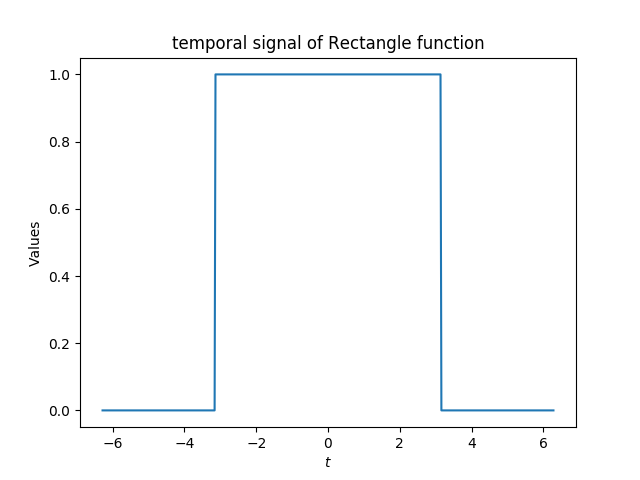
\includegraphics[width=0.45\textwidth]{python/Rectangular-Wave.png}
     \label{fig:SGD_1_single}}
     \quad 
     \subfigure[DFFT of $f(t)$]{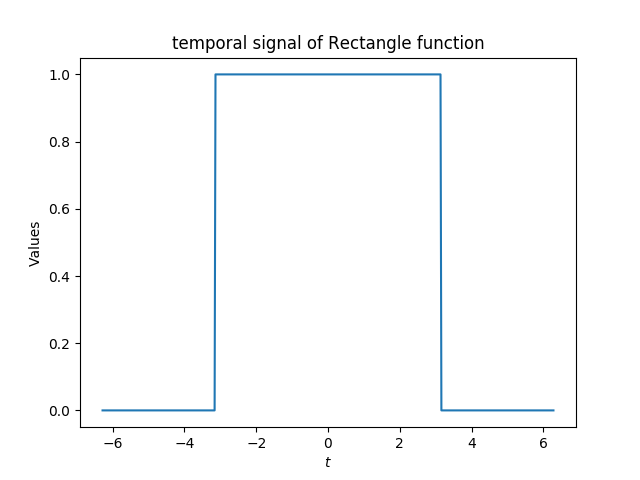
\includegraphics[width=0.45\textwidth]{python/Rectangular-Wave.png}
     \label{fig:SGD_1_single}} \\
     \subfigure[ $
     \widehat{f}(\lambda)$]{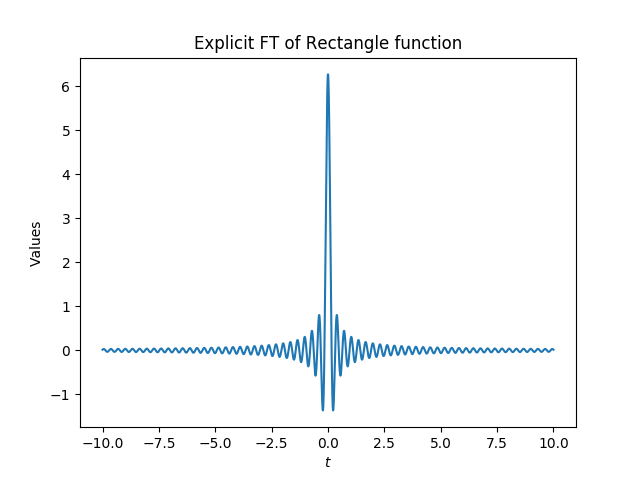
\includegraphics[width=0.45\textwidth]{python/ft-rectangle.png}
     \label{fig:SGD_1_single}}
 \end{figure*}


\end{exmp}


\begin{exmp}[$\cos(3t)$]
    
\begin{figure*}
     \centering 
    \subfigure[$\cos(3t)$]{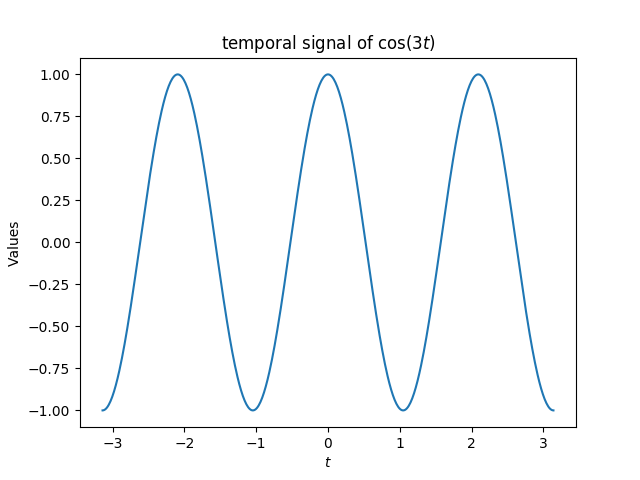
\includegraphics[width=0.45\textwidth]{python/cos3t.png}
     \label{fig:SGD_1_single}}
     \quad 
     \subfigure[DFFT of
     $f(t)$]{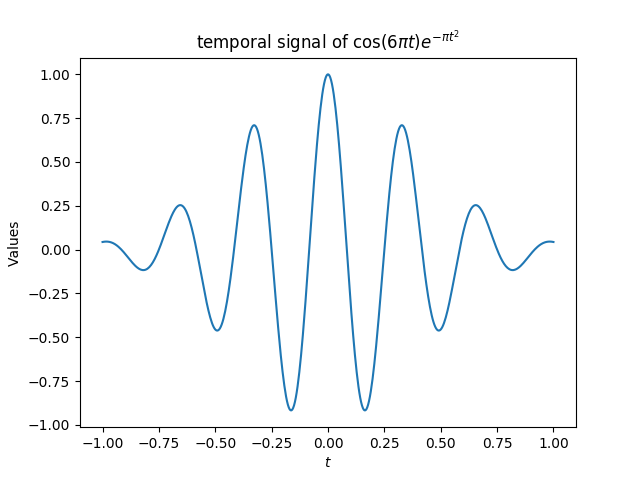
\includegraphics[width=0.45\textwidth]{python/cos-exp.png}
     \label{fig:SGD_1_single}} \\
     \subfigure[ $
     \widehat{f}(\lambda)$]{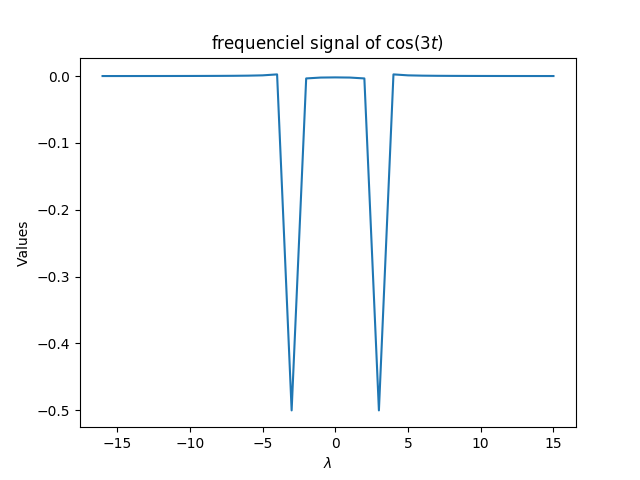
\includegraphics[width=0.45\textwidth]{python/fftcos3t.png}
     \label{fig:SGD_1_single}}
 \end{figure*}
\end{exmp}


\begin{exmp}[$\cos(6\pi t)e^{-\pi t^2}$]

\begin{figure*}
     \centering 
    \subfigure[Rectangle Function $f(t)$]{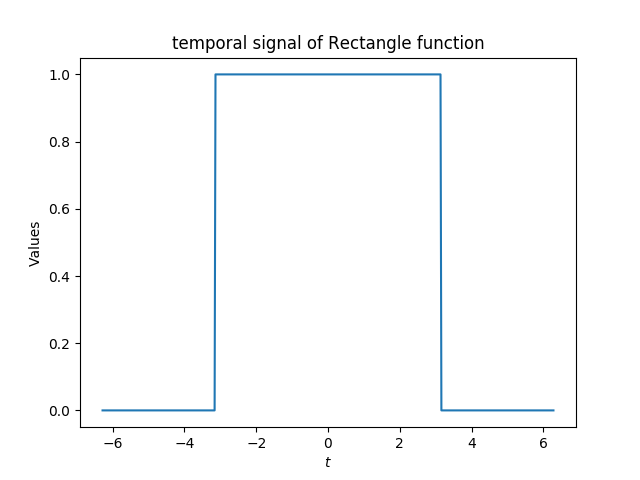
\includegraphics[width=0.45\textwidth]{python/Rectangular-Wave.png}
     \label{fig:SGD_1_single}}
     \quad 
     \subfigure[DFFT of $f(t)$]{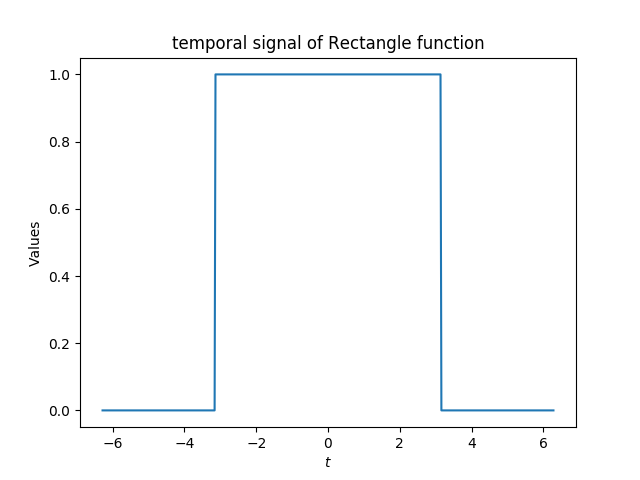
\includegraphics[width=0.45\textwidth]{python/Rectangular-Wave.png}
     \label{fig:SGD_1_single}} \\
     \subfigure[ $
     \widehat{f}(\lambda)$]{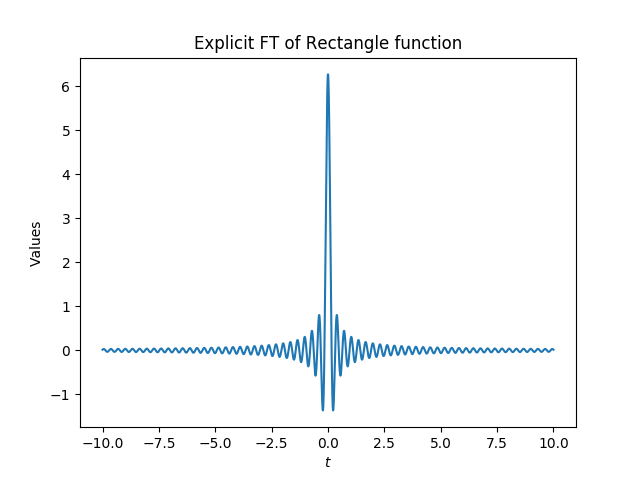
\includegraphics[width=0.45\textwidth]{python/ft-rectangle.png}
     \label{fig:SGD_1_single}}
 \end{figure*}
    
\end{exmp}

























\newpage

What is $ f_n  = f\left( \frac{ kT _{ \text{obs}  }^{  }  }{ N } \right)  $.  and what is
it to mean that the step is always 1/T for the DFT? 

\section{Properties of $ \mathscr{ FT }  $ on $ \mathscr{ L } ( \mathbb{R}) $ }
\label{sec:Properties of $ \mathscr{ FT }  $ on $ \mathscr{ L } ( \mathbb{R}) $ }
\begin{ftheo}[Exchange Property]
    Assume $ f, g\in \mathscr{L}^1( \mathbb{R})    $
    Then 
    \[
        \int\limits_{-\infty}^{\infty} f(u) \widehat{g}(u) \ du =
        \int\limits_{-\infty}^{\infty} \widehat{f}(u)g(u) \ du 
    \]
    \label{theo:Exchange Property}
\end{ftheo}

\begin{proof}
    $ -f \in \mathscr{L}^1, \widehat{g} \in \mathscr{ C } ^{\infty} \implies f\widehat{g}
    \in \mathscr{L}^1 $ then use fubini's theorem. 
\end{proof}


\subsection{FT and Derivation}
\label{subsec:FT and Derivation}
\begin{enumerate}
    \item Assume $ x^kf(x) $ in $ \mathscr{L}^1\left( \mathbb{R}\right)   $ 
        for $ k\in \set{ 0,\cdots,n }  $. Thus $ \widehat{f}  $ is k times derivable and 
\[
    \widehat{f} _{  }^{ (k) } (\lambda) = \widehat{\left( -2i\pi x\right) ^k f(x) } \left(
    \lambda \right) 
\]
    \item Assume $ f\in \mathscr{ C } ^n $ and $ f', \cdots, f^{(n)} \in
        \mathscr{L}^1\left( \mathbb{R}\right)  $.
    Then 
    \[
        \widehat{f^{(k)}}\left( \lambda \right) = \left( 2i\pi\lambda \right) ^k
        \widehat{f}\left( \lambda\right) 
    \]
    \item $ f\in \mathscr{L}^1\left( \mathbb{R}\right),\ f   $ bounded support then $
        \widehat{f} \in \mathscr{ C } ^{\infty}  $
\end{enumerate}
\begin{proof}
    \begin{enumerate}
        \item Direct application of the theorem of derivation 
            \[
            \int\limits_{ }^{ } \frac{ \partial  }{ \partial \lambda  } f\left( \lambda,
            t\right)  = \frac{ \partial  }{ \partial \lambda  } \int\limits_{ }^{ }
            f(\lambda, t) \ dt
            \]
        \item $ n = 1 $. $ f' \in \mathscr{L}^1\left( \mathbb{R}\right)   $. 
            \[
                \widehat{f'}\left( \lambda\right) = \lim_{a\to\infty}
                \int\limits_{a}^{a} e^{ -2i\pi\lambda t} f'(t) \ dt 
            \] integration by parts 
            \[
                \widehat{f'}\left( \lambda \right) = \lim_{a\to\infty} \left[ e^{
                -2i\pi\lambda t} f(t)  \right] ^a_{-a} + \lim_{a\to\infty}
                \int\limits_{-a}^{a } 2i\pi\lambda e^{ -2i\pi \lambda t } f(t) \ dt       
            \]
            \[
                \lim_{a\to\infty} \left[ e^{ -2i\pi\lambda t} f(t) \right] _{ -a }^{ a }  
            \]
            \[
                \lim_{a\to\infty} f(t) = 0 \quad \text{ since } \quad f\in
                \mathscr{L}^1p\left( \mathbb{R}\right) .  
            \]
            So, 
            \[
                \widehat{f'}\left( \lambda \right) = 2i\pi\lambda \widehat{f}\left(
                \lambda \right) 
            \]

     \item $ f\in \mathscr{L}^1\left( \mathbb{R}\right)  $ and $ f $ has a bounded
         support. Then what can we say about $ t^kf(t)  $. It is also in $
         \mathscr{L}^1\left( \mathbb{R}\right)   $ and using point 1 we get that $ f\in
         \mathscr{ C } ^{\infty}  $
    \end{enumerate}
\end{proof}
\subsection{Notations}
\label{subsec:Notations}
\begin{itemize}
    \item[symmetry] : 
        \[
            f _{ \sigma }^{  } (x) = f(-x) 
        \]
    \item[Translation] : 
        \[
        \mathscr{ T } af(x) = f(x-a) 
        \]
\end{itemize}



\subsection{Properties}
\label{subsec:Properties}
Assume f in L1 and $ \widehat{f}\left( \lambda \right) = \mathscr{ F } f(\lambda)  $. 
\begin{enumerate}
    \item $\overline{ \mathscr{ F } f} = \overline{ \mathscr{ F } } \overline{f} $
    \item $\left( \mathscr{ F } f\right) _{\sigma} = \overline{ \mathscr{ F } } f =
        \mathscr{ F } f_{\sigma} $
    \item $ f $ even $ \implies  \widehat{f} $ even 
    \item $ f $ odd $ \implies  \widehat{f} $ odd 
    \item $ f $ real and even then $ \widehat{f}  $ real and even   
    \item $ \widehat{ \mathscr{ T } a f}\left( \lambda \right) = e^{ -2i\pi\lambda a}
        \widehat{f}(\lambda)  $ time delay
    \item $ \mathscr{ T } a \widehat{f}\left( \lambda\right) = \widehat{ e^{ 2i\pia t}f(t)
        }\left( \lambda \right)   $ frequency delay
\end{enumerate}

\subsection{Usual examples}
\label{subsec:Usual examples}
\begin{align*}
    e^{ -ax} u(x) &= \frac{ 1 }{ a+2i\pi\lambda  }  \\ 
    e^{ ax} u(-t)  &= \frac{ -1 }{ -a + 2i\pi\lambda}  \\ 
    \frac{ x^k }{ k! } e^{ -ax} u(x)  &=  \frac{ 1 }{ \left( a + 2i\pi\lambda \right)
    ^{k+1}  } \\ 
        \frac{ x^k }{ k! } e^{ax} &= \frac{ -1 }{ \left(-a + 2i\pi\lambda\right)^{k+1}  }  \\ 
        e^{ -a \left | x \right | }  &= \frac{ 2a }{ a^2 + 4\pi^2\lambda^2 }  \\ 
        sign(x) e^{ -a \left | x \right | }  &= \frac{ -4i\pi\lambda }{ a^2 +
        4\pi^2\lambda^2 }  \\
            e^{-at^2} /& \sqrt{ \frac{ \pi }{ a } } e^{ \frac{ -\pi^2 }{ a^2 } \lambda^2}    \\
            \chi _{[-a, a]} (t)  &= \frac{ \sin(2a\pi\lambda)  }{ \pi x }  \\ 
\end{align*}

\subsection{Inverse of FT}
\label{subsec:Inverse of FT}
\begin{ftheo}[Inverse of FT]
    If $ f \in \mathscr{L}^1\left( \mathbb{R}\right)   $ and $ \widehat{f} \in
    \mathscr{L}^1\left( \mathbb{R}\right)   $. Then 
    \[
        \overline{ \mathscr{ F } } \widehat{f}(t) = f(t) , \quad \forall t \text{ where f
        cont} 
    \]
    But, $ f\in \mathscr{L}^1\left( \mathbb{R}\right) notimply \widehat{f} 
    \mathscr{L}^1\left( \mathbb{R}\right)   $ 
    \label{th:Inverse of FT}
\end{ftheo}

\begin{cor}[]
    $ f \in \mathscr{L}^1\left( \mathbb{R}\right)   $ and $ f \in \mathscr{ C } ^2  $ and
    $ f, f', f'' \in \mathscr{ L } ^1 $. Then 
    \[
        \widehat{f} \in \mathscr{L}^1\left( \mathbb{R}\right) .  
    \]
\end{cor}

\begin{proof}
    \[
        \widehat{f''}\left( \lamda \right) = -4\pi^2\lambda^2 \widehat{f}(\lambda) 
    \]
    and 
    \[
        \lim_{ \left | \lambda  \right | \to \omega } \left | \widehat{f''} \left( \lambda
        \right)  \right | = 0
    \] 
    Then 
    \[
    \exists M s.t. \left | \lambda  \right | > M \implies 4\pi^2\lambda^2 \left |
    \widehat{f} \left( \lambda \right)  \right | < 1
    \]
    $ \left | \widehat{f} \right | $ is continuous (RL theom). 
    \[
        \text{At } \omega \quad \left | \widehat(\lambda)  \right | < \frac{ 1 }{
        4\pi^2\lambda^2 } 
    \]
    Then 
    \[
        \left | \widehat{f}  \right | \in \mathscr{L}^1\left( \mathbb{R}\right)  
    \]
\end{proof}


\begin{cor}[]
    $ f, \widehat{f} \in \mathscr{L}^1  $, we have 
    \[
        \mathscr{ F } \widehat{f}\left( u\right) = f _{ \sigma  }^{  } (u) = f(-u) 
    \]
\end{cor}

\begin{exmp}[]
    Consider the previous examples. 
    \[
        \frac{ 1 }{ \left( a + 2i\pi t \right) ^{k+1}  } = \frac{ \left( -\lambda\right)
        ^k  }{ k! } e^{ a\lambda } u\left( -\lambda \right) 
    \]
    Also, 
    \[
        \frac{ -1 }{ \left( -a + 2i\pi t \right) ^{k+1}  } = \frac{ \left( -\lambda\right)
        ^k }{ k!  }e^{-a\lambda} u(\lambda)
    \]
    And 
    \[
    \frac{ 1 }{ a^2 + t^2  } = \frac{ \pi }{ a } e^{ -2i\pi \left | \lambda  \right | } 
    \]
\end{exmp}



\section{FT on $ \mathscr{ S } \left( \mathbb{R}\right)  $ }
\label{sec:FT on $ \mathscr{ S } \left( \mathbb{R}\right)  $ }
We need to restrict $ \mathscr{L}^1\left( \mathbb{R}\right)   $ in order to 
\begin{itemize}
  \item inverse FT
  \item Use derivation formulas 
\end{itemize}
In order to do this we use the Schwartz space. 
\begin{exmp}[Schwartz space ]
    \[
    \mathscr{ S } \left( \mathbb{R}\right) \subset \mathscr{L}^1\left( \mathbb{R}\right)  
    \]. 
\end{exmp}

\begin{defn}[Rapidly Decreasing Functions]
    \[
        \forall p \in \mathbb{N}, \lim_{p \to \infty} \left | x^p f(x)  \right | = 0
    \]
    \label{def:Rapidly Decreasing Functions}
\end{defn}

\begin{ftheo}[Property 1]    
If $ f \in \mathscr{L}^1\left( \mathbb{R}\right)  $ and is a rapidly decreasing function,
then 
\begin{enumerate}
    \item $ \forall p, t^pf(t) \in \mathscr{L}^1\left( \mathbb{R}\right)   $
    \item $ \widehat{f} \in \mathscr{ C } ^{\infty}  $
\end{enumerate}
    \label{th:}
\end{ftheo}
\begin{proof}
    $ f $ is rapidly decreasing. 
    \[
        \implies \forall p \in \mathbb{N} \quad \lim_{ \left | x \right | \to \infty}
        \left | x^{p+2} f(x)  \right | = 0
    \]
    \[
        \imples \exists M s.t. \left | x \right | > M  \quad \left | x^{p+2} f(x)  \right
        | < 1   
    \]
    \[
    \int\limits_{ }^{ } \left | x^p f(x)  \right | \ dx = \int\limits_{ \left | x \right |
    < M }^{ } \left | x^p f(x)  \right | \ dx + \int\limits_{ \left | x \right | > M
}^{}  + \int\limits_{ \left | x \right | > M }^{ } \frac{ 1 }{ x^2  } \left | x^{p+2} f(t)
\right | \ dt 
    \]
    \[
        \leq M^p \int\limits_{ \left | x \right | < M }^{ } \left | f(x)  \right | \ dx +
        \int\limits_{ \left | x  \right | > M }^{ } \frac{ 1  }{ x^2  } \ dx
    \]
    \[
    \leq \infty 
    \]
    Then $ \forall p, \quad x^p f(x) \in \mathscr{L}^1\left( \mathbb{R}\right)   $. 
    Then
    \[
        \widehat{ \left( -2i\pi t \right) ^k f(t) } 
    \] exisits and it is $ \widehat{f}^{(k)} \left( \lambda \right)  $

\end{proof}

\begin{ftheo}[Property 2]
    Let $ f \in \mathscr{ C } ^{\infty}  $ and $ \forall k  $ $ f^{(k)} \in
    \mathscr{L}^1\left( \mathbb{R}\right)   $. Then $ \widehat{f}  $ is rapidly
    decreasing.     
    \label{th:Property 2}
\end{ftheo}
\begin{proof}
    \[
        \widehat{f _{  }^{ (k) } }\left( \lambda \right) = \left( 2i\pi\lambda \right) ^k
        \widehat{f} \left( \lambda \right)          
    \]
    By RL theorem 
    \[
        \lim_{ \left | \lambda  \right | \to \infty} \left | \widehat{f _{  }^{ (k)  } }
         (\lambda)  \right| = 0  
    \]
    Then 
    \[
        \lim_{ \left | \lambda  \right | \to 0} \left | \lambda^k \widehat{f}(\lambda)
        \right | = 0
    \]
\end{proof}
\subsubsection{Conclusion }
The more regular $ f  $ is, the more rapidly $ \widehat{f}  $ converges to zero at
infinity. The more rapidly $ f $ converges, the more regular $ \widehat{f} $ is. 
Furthermore, we realize that if $ f \in \mathscr{ C } ^{\infty}  $ and $ f  $ rapidly
decreasing, then $ \widehat{f}  $ rapidly decreasing and $ \widehat{f} \in \mathscr{ C }
^{\infty}   $. 

\begin{defn}[Schwartz Space]
    The vectorial space $ \mathscr{ S } \left( \mathbb{R}\right)  $ of function are those
    function for which 
    \[
     f \in \mathscr{ C } _{  }^{ \infty }  
    \]
    \[
     f _{  }^{ (k)  } \text{ are rapidly decreasing for all k}  
    \]
    \label{def:Schwartz Space}
\end{defn}

We have for $ \mathscr{ S } \left( \mathbb{R}\right) \subset \mathscr{L}^1\left( \mathbb{R}\right)   $
\begin{enumerate}
    \item $ \mathscr{ S }  $ stable for derivatives 
    \item $ \mathscr{ S }  $ stable for $ \mathscr{ FT }  $
    \item $ \mathscr{ S }  $ stable for x by a polynomial 
\end{enumerate}

$ \mathscr{ FT }  $ is a bijection from $ \mathscr{ S } \left( \mathbb{R}\right)  $ to
itself. 

\chapter{FT on $ \mathscr{L}^2(\mathbb{R} )    $}
In signal processing, we often work with 
\[
\int\limits_{ }^{ } \left | f(t)  \right | ^2 \ dt = \text{ the energy of the signal} =
\|f\|_{2} 
\]
$ \mathscr{L}^2(\mathbb{R})  $ is the "natural" space for signals. To define $ \mathscr{
FT }  $ on $ \mathscr{L}^2(\mathbb{R})  $, we use the density of $ \mathscr{ S } \left(
\mathbb{R}\right)  $ in $ \mathscr{L}^2(\mathbb{R})  $.
\begin{ftheo}[Extension Theorem]
    $ E, F $ vectorial spaces with norm. F is complete. Let G be a dense subspace of E.
    Let A be a linear continuous application from G to F. Then $ \exists ! $ extension of
    $ A : E \to F  = \overline{A} $. $ \overline{A} $ is lin and cont and $ \|
    \overline{A} \|^{ }_{ E, F} = \| A \|^{ }_{ G, F}  $. With 
    \[
    \| A \|^{ }_{ G, F} = Sup \left( \frac{ \| A f \|^{ }_{ F}  }{ \| f \|^{ }_{ G}  } \right) 
    \]
    \label{th:Extension Theorem}
\end{ftheo}


\section{Properties of $ \mathscr{ FT }  $ on $ \mathscr{L}^2(\mathbb{R})  $}
\label{sec:Properties of $ \mathscr{ FT }  $ on $ \mathscr{L}^2(\mathbb{R})  $}
\begin{enumerate}
    \item $ \forall f\in \mathscr{L}^2(\mathbb{R})  $. $ \mathscr{ F\overline{F} } f =
        \mathscr{ FF } f = f $ almost everywhere.
    \item $ \forall f,g \in \mathscr{L}^2(\mathbb{R}) \times \mathscr{L}^2(\mathbb{R})  $. 
        \[
            \int\limits_{ }^{ } f(t) \overline{g}(t) \ dt = \int\limits_{ }^{ } \mathscr{
            F} f(\lambda) \overline{ \mathscr{ F } g} \left( \lambda \right) \ d\lambda 
        \]
        \[
            \langle f,g \rangle _{ L^2 }^{  } = \langle \widehat{f} , \widehat{g}  \rangle
            _{ L^2 }^{  } 
        \]
    \item 
        \[
            \| f \|^{ }_{ 2} = \| \widehat{f} \|^{ }_{ 2} 
        \]
        energy conservation or Parseval equality. 
    \item Exchange property. $ f,g \in \mathscr{L}^2(\mathbb{R}) \times \mathscr{L}^2(\mathbb{R})  $
        \[
            \int\limits_{ }^{ } f(u) \widehat{g}(u) \ du = \int\limits_{ }^{ }
            \widehat{f}(u) g(u) \ du 
        \]
\end{enumerate}
\begin{exmp}[]
    We can do IFT on the functions listed previously to see if we can perform the IFT. 
\end{exmp}

\section{FT and Convolution}
\label{sec:FT and Convolution}
\subsubsection{Part A}

$ f,g \in \mathscr{L}^2\left( \mathbb{R}\right)   $. 
Then 
\begin{enumerate}
    \item $\widehat{f*g} \left( \lambda \right) = \widehat{f}(\lambda) \cdot
        \widehat{g}(\lambda)  $
    \item $ \widehat{f \cdot g} \left( \lambda \right) = \widehat{f} * \widehat{g} \left(
        \lambda \right)  $
\end{enumerate}

\subsubsection{Part B}
$ f, g \in \mathscr{ S } \left( \mathbb{R}\right)  $, then 
\begin{enumerate}
    \item $\widehat{f*g} = \widehat{f}\cdot\widehat{g} $
    \item $\widehat{f\cdot g} = \widehat{f} * \widehat{g}$
\end{enumerate}

\subsubsection{Part C}
$ f,g \in \mathscr{L}^2(\mathbb{R})  $
\begin{enumerate}
    \item $f * g(t) = \overline{F}\left( \widehat{f} \widehat{g}\right) (t) $
    \item $ \widehat{f\cdot g} = \widehat{f} * \widehat{g} (\lambda) $
\end{enumerate}


\section{Heisenberg Uncertainty Principle}
\label{sec:Heisenberg Uncertainty Principle}
\subsection{Exercises}
\label{subsec:Exercises}

\subsection{Interpretation of Heisenberg's Uncertainty Principle}
\label{subsec:Interpretation of Heisenberg's Uncertainty Principle}
Let $ f(t)  $ be our signal and $ \widehat{f}(\lambda) $ be its frequential
representation. We say that 
\[
    \int\limits_{ }^{ } \left | f(t) \right | \ dt = \int\limits_{ }^{ } \left |
    \widehat{f}(\lambda) \right |^2 \ dt
\] is the energy of the signal and $ \left | f(t)  \right | ^2 $ is the local density. 
\begin{itemize}
  \item We can view a signal as its density of energy. 
  \item We can summarize $ f(t)  $ by the box there is between time and frequency
      accuracy. 
      \[
          \mu_N : \sigma_t\sigma_{\epsilon} > \frac{ 1 }{ 4\pi } 
      \]
\end{itemize}

\begin{figure}[ht]
    \centering
    \incfig{heisunbox}
    \caption{heisUnBox}
    \label{fig:heisunbox}
\end{figure}

\section{Conclusion About Fourier Transform}
\label{sec:Conclusion About Fourier Transform}
Very useful because  : 
\begin{enumerate}
    \item Transform Convolution into product
    \item Transforms derivative into polynomial
    \item Easy to compute using the FFT algorithm
\end{enumerate}
But, this is a tool adopted for the use of "regular" signals, stationary signals. The tool
is not performed for iregular sizes. Example : 
Show $ \delta_0  $ and its fourier Transform. 

Consider 
\[
    f(t) = \left( \sin(2\pi 5t) + \sin(2\pi 20t) \right) \mathbbm{1}_{[0,1[} \text{ and } 
    g(t) = \sin(2\pi 5t) \mathbbm{1}_{[0,\alpha[} + \sin(2\pi 20t)\mathbbm{1}_{[\alpha,1[} 
\]

Use graphs from python to explain! 

To correct these drawbacks. We use 
\begin{itemize}
  \item Window Fourier Transform
  \item Gabor Transform
  \item Continuous Wavelet Transform and Discrete Wavelet Transform
\end{itemize}




\chapter{Window Fourier Transform} 
\begin{figure}[ht]
    \centering
    \incfig{wftonf}
    \caption{WFT of $f$}
    \label{fig:wftonf}
\end{figure}

\begin{defn}[Window]
    Let $ w $ a window such that $ w \in \mathscr{L}^2 \wedge \mathscr{L}^2 $ and $ \left
    | \widehat{w} \right |  $ is an odd function and $ \| w \|^{ }_{ 2} = 1 $
    We define 
    \[
        w _{ \lambda, b }^{  } (t) = w(t-b) e^{ 2i\pi\lambda t} 
    \]
    then $ \forall f \in \mathscr{L}^2(\mathbb{R})   $ the WFT is defined as 
    \[
        W_f(\lambda,b) = \int\limits_{-\infty}^{\infty} f(t) \overline{w}_{\lambda, b}(t)
        \ dt 
    \]
    \label{def:Window}
\end{defn}

Some properties 
\begin{enumerate}[label={(\alph*)}]
    \item Conservation of Energy : 
        \[
            \int\limits_{-\infty}^{\infty} \left | f(t)  \right | ^2 \ dt =
            \int\limits_{-\infty}^{\infty} \int\limits_{-\infty}^{\infty} \left |
            W_f\left( \lambda, b\right)  \right | ^2 \ d\lambda \ db
        \]
    \item Reconstruction formula : 
        \[
            f(x) = \int\limits_{-\infty}^{\infty} \int\limits_{-\infty}^{\infty}
            W_f(\lambda, b) w_{\lambda, b} (t) \ d\lambda \ db
        \]
\end{enumerate}
\subsubsection{Comment:}
How to choose $ w $? In practice $ w $ is centered and symmetric on 0. We want $
w_{\lambda, b}(t) $ centered on $ \left( \lambda, b\right)  $. 
\section{Exercises : Atoms}
\label{sec:Exercises : Atoms}
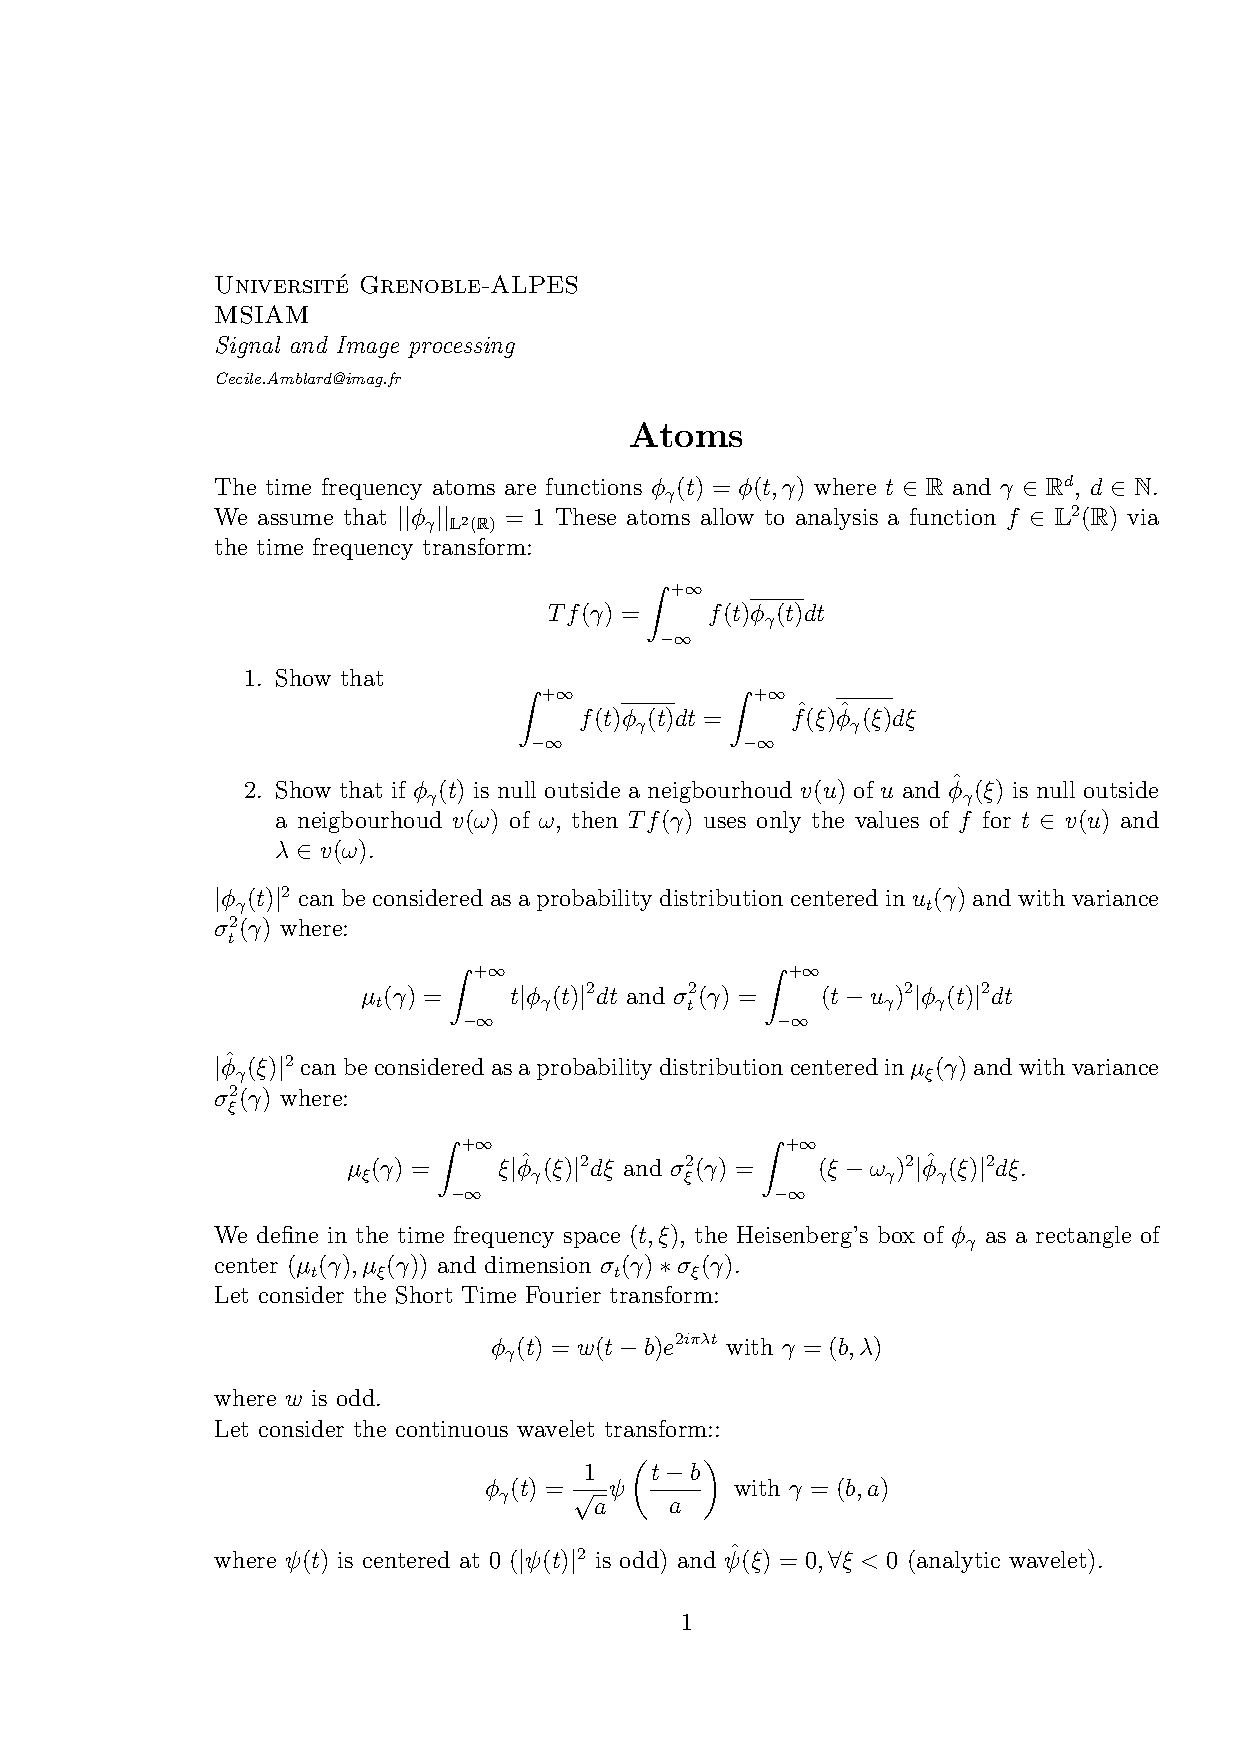
\includepdf[pages=-]{References/TDTempsFreq.pdf} 
\subsubsection{Part 1)}


\subsubsection{Part 2)}
\begin{align*}
    \mu_t(\gamma) &= \int\limits_{-\infty}^{\infty} t \left | \phi_{\gamma}(t) \right | ^2
    \ dt \\
                  &= \int\limits_{-\infty}^{\infty} t \left | w(t-b) e^{ 2i\pi\lambda t}  \right | ^2
    \ dt \\
                  &= \int\limits_{-\infty}^{\infty} (u+b) \left | w(u)\right | ^2\ du \\
                   &= b \text{ since } \| w \|^{ }_{ 2} = 1; \| w \|^{ 2}_{ } \text{ is
                   even }
\end{align*}

\begin{align*}
    \sigma_t^2 &= \int\limits_{-\infty}^{\infty}\left( t-\mu_t\right) ^2 \left |
    \phi_{\gamma} (t) \right | ^2 \ dt \\ 
 &= \int\limits_{-\infty}^{\infty} \left( t-b\right) ^2 \left | w\left( t-b\right)  \right
 | ^2 \ dt \\ 
 &= \int\limits_{-\infty}^{\infty} u^2 \left | w(u) \right | ^2 \ du \\ 
  &= \sigma^2_w \\ 
\end{align*}

\begin{align*}
    \widehat{\phi}(\xi) &= \int\limits_{-\infty}^{\infty} \phi_{\gamma}(t) e^{ -2i\pi\xi t}
    \ dt \\
     &= \int\limits_{-\infty}^{\infty} w(t-b) e^{ -2i\pi t(\xi - \lambda) } \ dt \\
     &= \int\limits_{-\infty}^{\infty} w(u) e^{ -2i\pi(u+b)(\xi-\lambda)} \ du \\
     &= e^{ 2i\pib(\lambda-\xi)} \int\limits_{-\infty}^{\infty} w(u) e^{ -2i\pi u (\xi -
     \lambda) } \ du  \\
     &= e^{ 2i\pi b (\lambda - \xi) } \widehat{w}(\xi - \lambda)
\end{align*}
and we have that 
\begin{align*}
    \left | \phi_{\gamma}(\xi) \right |  &= \left | \widehat{w}\left( \xi - \lambda\right)
    \right |\ d\xi   \\ 
    \mu_{\xi}  &= \int\limits_{-\infty}^{\infty}  \xi \left | \widehat{w}\left( \xi -
    \lambda\right)  \right |^2 \ d\xi  \\ 
               &= \int\limits_{-\infty}^{\infty} \left( f + \lambda \right) \left |
               \widehat{w}(f) \right | ^2 \ df \\ 
                &= \lambda  \\ 
\end{align*}
Finally, this all implies that 
$ \sigma _{ \xi }^{ 2 }  = \int\limits_{-\infty}^{\infty} f^2 \left | \widehat{w}(f)
\right | ^2 \ df = \sigma _{ \widehat{w}  }^{ 2 } $. 
$ \\ $
$ w_{\gamma}  $ is a signal whose energy can be represented by a box, like
\ref{fig:heisunbox}, if $ \gamma  $ changes, the center of the box changes but the
dimension of the box does not change. Atoms $ \phi_{\gamma}  $ are represented by temporal
spatial boxes of the same size. If the lengths of support of $ \phi_{\gamma}  $ is not
large enough, we can't capture low frequency. If the length of the support is too large,
we analyze high frequency component of the signal but lose time accuracy.

\chapter{Continuous Wavelet Transform} 
\subsubsection{Motivations}
We want to analyze a signal through atoms whose dimensions changes versus frequencies. 
\begin{defn}[Analyzing function]
    The continuous wavelet transform uses an analyzing function
    \[
        \psi_{a,b}(t) = \frac{ 1 }{ \sqrt{a}  } \psi \left( \frac{ t-b }{ a } \right) 
    \]
    where b is the translation parameter and a is the scale parameter. 
    \label{def:Analyzing function}
\end{defn}
For each $ \psi  $ there exists an exact link between scale and frequency. 
\begin{figure}[ht]
    \centering
    \incfig{psinormal}
    \caption{$\psi_{[1,0]}$ }
    \label{fig:psinormal}
\end{figure}

\begin{figure}[ht]
    \centering
    \incfig{psistretch}
    \caption{Dilation}
    \label{fig:psistretch}
\end{figure}

\begin{figure}[ht]
    \centering
    \incfig{contraction}
    \caption{contraction}
    \label{fig:contraction}
\end{figure}
\newpage
High scale captures low frequencies, and low scale saptures hight frequency. 

$ \\ $
\newpage
\begin{defn}[Wavelet]
    Let $ \psi \in \mathscr{L}^1(\mathbb{R}) \cap \mathscr{L}^2(\mathbb{R})   $ such that 
    \begin{enumerate}
        \item \[
                \int\limits_{-\infty}^{\infty} \frac{ \left | \widehat{\psi}(\lambda)
                \right | ^2}{ \left | \lambda  \right | }\ d\lambda = K < \infty
        \]
    \item $ \| \psi \|^{ }_{ 2} = 1 $. 
    \end{enumerate}
    Let 
    \[
        \psi_{a,b}(t) = \frac{ 1 }{ \sqrt{a}  } \psi \left( \frac{ t-b }{ a } \right) 
    \] and $ \forall f \in \mathscr{L}^2(\mathbb{R})$ we consider the coefficients of an
    ondelette to be given by 
    \[
        C_f(a,b) = \int\limits_{-\infty}^{\infty} f(t) \overline{\psi}_{a,b}(t) \ dt
    \]
    \label{def:Wavelet}
\end{defn}

We have the following properties. 
\begin{enumerate}[label={(\alph*)}]
    \item Conservation of Energy : 
        \[
        \frac{ 1 }{ K } \int\limits_{-\infty}^{\infty} \int\limits_{-\infty}^{\infty}
        \left | C_f(a,b)  \right | ^2 \frac{ dadb }{ a^2  }
        \]
    \item Reconstruction Formula : 
        \[
            \frac{ 1 }{ K } \int\limits_{-\infty}^{\infty} \int\limits_{-\infty}^{\infty}
            C_f(a,b) \psi_{a,b} (x) \frac{ dadb }{ a^2 } 
        \]
\end{enumerate}
In practice we choose $ \psi $ such that $ \widehat{\psi}(0) = 0 $ oscilating function. 

Give the formulas and graphs for Haar wavelet, Mexican Hat, and Morlet wavelet. 

\subsection{Problem #?}
\label{subsec:Problem #?}
\begin{align*}
    \psi_{a,b} &= \frac{ 1 }{ \sqrt{a}  } \psi\left( \frac{ t-b }{ a } \right) 
\end{align*}
\begin{align*}
    \mu_t(\gamma)  &= \int\limits_{-\infty}^{\infty} t \left | \phi_{\gamma} (t) \right |
    ^2 \ dt \\ 
     &= \int\limits_{-\infty}^{\infty} t \left | \frac{ 1 }{ \sqrt{a}  } \psi\left( \frac{ t-b }{ a } \right)\right |^2 \ dt \\  
      &u = \frac{ t-b }{ a }  \implies t = au+b \text{ and } dt = a \ du\\ 
      \mu_t &= \frac{ 1 }{ a } \int\limits_{-\infty}^{\infty} \left( au+b\right) \left |
      \psi_{a,b} (u)  \right | ^2 \ adu  \\
       &= b \text{ since } \psi \text{ even and  } \| \psi  \|^{ 2}_{ 2} = 1 \\ 
\end{align*}

\begin{align*}
    \sigma_t^2 &= \frac{ 1 }{ a } \int\limits_{-\infty}^{\infty} \left( t-b\right) ^2 \left
    | \psi \left( \frac{ t-b }{ a } \right)  \right | ^2 \ dt \\ 
     &= \int\limits_{-\infty}^{\infty} a^2 u^2 \left | \psi\left( u\right)  \right | ^2 \
     du \\ 
      &= a^2\sigma_4^2 \\ 
\end{align*}

\begin{align*}
    \widehat{\psi}_{a,b} (\lambda)   &= \frac{ 1 }{ \sqrt{a}  }
    \int\limits_{-\infty}^{\infty} \psi \left( \frac{ t-b }{ a }\right)   e^{
    -2i\pi\lambda t} \ dt  \\ 
                                     &= \sqrt{a} 
    \int\limits_{-\infty}^{\infty} \psi \left( u \right)   e^{
    -2i\pi\lambda[au+b] } \ dt  \\ 
                                     &= \sqrt{a} e^{ -2i\pi\lambda b} \psi(a\lambda)  \\ 
\end{align*}

\begin{align*}
    \mu_{\xi}(\gamma) &= \int\limits_{-\infty}^{\infty} \lambda a \left |
    \widehat{\psi}\left( a\lambda\right)  \right | ^2 \ d\lambda \\ 
                      &= \int\limits_{-\infty}^{\infty} f \left | \widehat{\psi} (f)
                      \right | ^2 \frac{ df }{ a }  \\ 
                       &= \frac{ 1 }{ a } \int\limits_{-\infty}^{\infty} f \left |
                       \widehat{\psi} (f)  \right | ^2 \ df  \\ 
                        &= \frac{ ?  }{ a }  \\ 
\end{align*}
Where $ ?   $ is maybe $ \Gamma $
The previous calculation shows that frequency is the inverse of scale. 

\begin{align*}
    \sigma _{ \xi }^{ 2 } (\gamma)  &= \int\limits_{-\infty}^{\infty} \left( \lambda -
    \frac{ \Gamma  }{ a } \right) a \left | \widehat{\psi} (a\lambda)  \right | ^2 \
    d\lambda  \\ 
     &= \int\limits_{-\infty}^{\infty} \left( \frac{ f - \Gamma }{ a } \right) ^2 \left |
     \widehat{\psi} (f)\right | ^2 \ df   \\ 
      &= \frac{ 1 }{ a^2 } \int\limits_{-\infty}^{\infty} \left( f - \Gamma\right) ^2
      \left | \widehat{\psi}(f) \right | ^2 \ df = \frac{ 1 }{ a^2  } \sigma _{
      \widehat{\psi} }^{ 2 }  \\ 
\end{align*}





\section{Random Discussion}
\label{sec:Random Discussion}
We have that
\[
\int\limits_{ }^{ } \left | f(t)  \right | ^2 \ dt  
\]
gives us the energy density which we can think of as a probability density. 
Think about the frequency space 

In Window Fourier transform, the dimension of boxes are independent of position $ \left( \mu_t,
\mu_\xi \right)  $ of the 

In continuous wavelet transform 
dimension of $ \sigma  $ on the scale $ a $. 

The aim of CWT is to analyze non-stationary signals that have height variations with less
regularity. 

\section{Intro}
\label{sec:Intro}
\section{Definition and reconstruction theroem}
\label{sec:Definition and reconstruction theroem}

\section{Properties Or how to choose $ \psi $ }
\label{sec:Properties}
Many possible choices for function $ \psi \in \mathbb{R} \text{ or } \mathbb{C} $ and
analytic. There is a link between regularity of the signal to analyze $ f $ and the
wavelet transform $ Cf(a,b) $ This link is dependent on the number of null moments of $
\psi $.
\begin{ftheo}[]
    Let $ f\in \mathscr{ C } ^n $ and $ f _{  }^{ (n) }  $ is bounded and $ \psi  $ has n
    null moments 
    defined as 
    \[
        \int\limits_{ }^{ } t^k \psi (t) \ dt = 0 \quad \forall k \in \set{ 0,\cdots, n } 
    \]


    $ \\ $
    Then 
    \[
        \left | Cf(a,b)  \right | = k \left( a ^{n + 1/2}\right) \quad k \in \mathbb{R}
    \]
    \label{th:}
\end{ftheo}

\begin{proof}
   Let $ f \in \mathscr{ C } ^n $  thus we can expand this using Taylor's formula : 
   \[
       f(t) = \sum_{k=0}^{n-1} \frac{ f^{(k)} }{k!  } \left( t-u\right) ^k + \frac{
           f^{(n)}(c) }{ n! } (t-u)^n \quad u \leq c \leq t 
   \]
   \begin{align*}
       Cf(a,b) &= \frac{ 1 }{ \sqrt{a} } \int\limits_{ }^{ } f(t)\psi ( \frac{ t-b }{ a } )
       \ dt \\
       Cf(a,b) &= \sum_{k=0}^{n-1} \frac{ f^k(a) }{ k! } \int\limits_{}^{ } \left(
       t-u\right) ^k \psi\left( \frac{ t-b }{ a } \right) \frac{ dt }{ \sqrt{a} }\\ 
        &\text{ Let } x = \frac{ t-b }{ a }  \\ 
           Cf(a,b) &= \sum_{k=0}^{n-1} \frac{ f^{(k)}(u) }{ k! } \int\limits_{}^{} \left(
           ax+b - u \right) ^k \psi(x)\sqrt{a} \ dx + 
           \sqrt{a} \frac{ f^{(n)} (c) }{ n!  } \int\limits_{ }^{ } \left( ax + b -
           u\right) ^n \psi (x) \ dx 
       \end{align*}
       Using the fact that $ \forall 0 \leq k \leq n $ gives 
       \[
           \int\limits_{}^{ } t^k \psi(t) \ dt = 0
       \]
       we obtain 
      \[
          Cf(a,b) = \sqrt{a} \frac{ f^{(n)}(c) }{ n! } \int\limits_{ }^{ } \left( ax + b -
          u \right) ^n \overline{\psi}(x) \ dx 
      \] 
      using 
      \[
      \left( \alpha + \beta \right) ^n \leq 2^n\left( \left | a \right | ^n + \left | b
      \right | ^n \right) 
      \]
      then 
   %   \begin{align*}
   %       Cf(a,b) &\leq \frac{ f^{(n)} (c) 2^n a^{n+1/2} }{ n! } \int\limits_{ }^{ }\left|
   %       x^n \right| \left|\overbar{\psi}(x)\right| \ dx 
   %       +  \frac{ f^{(n)}(c)  }{ n! } 2^n\sqrt{a} \underbrace{\int\limits_{
   %           }^{ } \left | b-?\right| ^n \left | \overline{\psi}(x) \right | \ dx 
   %   \end{align*}
      if $ f\in \mathscr{ C } ^n $ we can choose $ u = b $ then 
      \[
          Cf(a,b) \leq k a^{n+1/2} 
      \] with 
      \[
          k = 2^n \frac{ \sup(f)^{(n)} }{ n! } \int\limits_{ }^{ } \left | x^n \right |
          \left | \overline{\psi}(x) \right | \ dx
      \]
\end{proof}
  \begin{enumerate}[label={(\alph*)}]
      \item $ \psi $ has p null moments $ p < n  $
      \item $ \psi  $ has p null moments $ p > n $
  \end{enumerate}
\[
    Cf(a,b) = \underbrace{\sum_{n-1}^{k=0} \frac{ f^{(k)(x) }{ k! } \int\limits_{ }^{ } \left(
            t-u\right) ^k \overline{\psi} \frac{ \left( t-b\right)  }{ a } \frac{ dt }{
    \sqrt{a}  }}_{S_n-1} + \frac{ f^{(n)}(c) }{ n! } \int\limits_{ }^{ } \left( t-u\right) 
\]
Case 1 : 
$ p < n  $ then $ S_n -1 \neq 0  $. 

$ \\ $

\subsection{Properties of $ \psi $}
$ \psi  $ can be either:  
\begin{itemize}
  \item  real or complex and either complex analytic or non-analytic. 
  \item Finite support of large size that scales with a
  \item $ \psi  $ can be "regular" 
  \item $ \psi $ can have $ n  $ null moments
\end{itemize}
a)
Look at the exercise 
\[
    f(t) = \cos 2\pi\lambda_0t 
\]
\subsection{Include Figures for Analytic vs. Non-analytic Functions}
\label{subsec:Include Figures for Analytic vs. Non-analytic Functions}


b)
$ Cf(a,b)  $ uses $ f(t_0)  $ if $ t_0 \in $ supp$(\psi_{a,b}) $ the number of values of
$ Cf(a,b)  $ which uses $ f\left( t_0 \right)  $ depends on the size of the support of $
\psi $. We don't want all $ Cf(a,b) $ to contain $ t_0 $ as we want differing information
for differening $ Cf(a,b) $.

\subsubsection{c) Regularity of $ \psi $}
Using the reconstruction formula, we write the reconstructed signal as a weighted sum of
$ \psi_{a,b}  $ where 
\[
    f(t) = \int\limits_{ }^{ } \int\limits_{ }^{ } Cf(a,b) \psi_{a,b} (t) \frac{ da\  db
    }{ a^2 } 
\]
In practice, the reconstructed signal is a finite sum of $ \psi_{a,b}  $. So if $
\psi_{a,b}  $ is not continuous $ f_r  $ wil be non continuous, for example : 
\subsection{Insert image of Haar wavelet reconstruction}
\label{subsec:Insert image of Haar wavelet reconstruction}

\[
    \psi (t) 
\]

\subsubsection{d) Number of Null Moments}
The speed of convergence of $ Cf(a,b) $ for $ a \to 0 $ depends on this number of null
moments. 

\begin{defn}[Lipshitz function]
    $ f $ is $ \alpha  $ Lipshitz at $ v  $, $ \alpha \geq 0  $ means 
    \[
        \exists P_v(t) = \sum_{k=0}^{m-1} \frac{ f _{  }^{ (k) } (v)  }{ k!  } \left( t-v
        \right) ^k 
    \] $ m = [\alpha]  $, then $ \forall t \in \mathbb{R} $ 
    \[
        \left | f(t) - P_v(t)  \right | \leq K \left | t-v  \right | ^{\alpha} 
    \]
    $ f $ is uniformly lipshitz in $ [a,b]  $ then $ \forall v \in [a,b] , \forall t \in \mathbb{R} $
    \[
        \left | f(t) - P_v(t)  \right | \leq K \left | t-v  \right | ^{\alpha} 
    \]
    \label{def:Lipshitz function}
\end{defn}

Also, if $ f = g'  $ with $ g $ being $ \alpha  $ Lipshitz, then $ f $ is $ \left( \alpha
-1 \right)  $ Lipshitz. 

\begin{exmp}[]
    \[
    \delta_0 = u' \text{ with ...} 
    \]
\end{exmp}



\begin{ftheo}[]
    $ \psi  $ has $ n  $ null moments 
    \[
        \forall k \in [0, n-1] , \ \int\limits_{ }^{ } t^k \psi(t) \ dt = 0
    \]
    $ f $ is $ \alpha  $ Liptshitz , $ \alpha < n  $ at $ v  $. 
    Then 
    \[
        \left | Cf(a,b)  \right | \leq Aa^{\alpha + 1/2 } \left( 1 + \left | \frac{ b-v
        }{ a }  \right | \alpha \right) 
    \]
    \label{th:}
\end{ftheo} 


\begin{proof}
    $ f(t) = P_v(t) + \Epsilon (t)  $ with $ \left | \Epsilon (t)  \right | \leq k \left |
    t-v \right |\alpha   $
    \[
        Cf(a,b) = \int\limits_{ }^{ } f(t) \psi_{a,b} )(t) \ dt 
    \]
    \[
        = \sum_{k=0}^{m-1} \frac{ f^{(k)} (v)  }{ k!  } \int\limits_{ }^{ } \left( t-v
        \right) ^k \psi_{a,b} (t) \ dt + \int\limits_{ }^{ } \Epsilon(t) \psi_{a,b} (t) \
        dt 
    \]
    Let $ x = \frac{ t-b }{ a }  $
    \[
        f(t) = \sum_{k=0}^{m-1} \frac{ f^{(k)}(v)  }{ k!  } \int\limits_{}^{ } \left( ax +
        b - v \right) ^k \psi(x) \sqrt{a} \ dx + \sqrt{a} \int\limits_{ }^{ } \Epsilon(ax
        + b - v) \psi(x) \ dx
    \]
    \[
        \left | Cf(a,b)  \right | \leq \sqrt{a} \int\limits_{ }^{ } \left | \Epsilon(ax +
        b - v) \right | \psi(x) \ dx 
    \]
    \[
        \leq \sqrt{a} K \int\limits_{ }^{ } \left | ax + b - v  \right | ^{\alpha} \psi(x)
        \ dx 
    \]
    $ \left | a+b \right | ^{\alpha}  \leq 2^{\alpha} \left( \left | a \right|^{\alpha} +
    \left | b \right | ^{\alpha} \right) $
    \[
        \left | Cf(a,b)  \right | \leq k2^{\alpha} \sqrt{a} \left( \int\limits_{ }^{ } a
        _{  }^{ \alpha  } \left | x \right | _{  }^{ \alpha  } \psi(x) \ dx + \left | b -
    v \right | _{  }^{ \alpha  } \left |\psi(x) \right | dx \right) 
    \]

\end{proof}


If $ \alpha = -1  $ at $ v  $, we have a strong singularity at $ v  $, which coefficients
$ Cf(a,b)  $ will be influenced by this. We search $ \set{ (a,b) | v \in \text{supp}
\psi_{a,b} }  $. Consider $ \text{supp} \left( \psi \right) = [-c, c]  $ then 
\[
    \set{ (a,b) \bracevert v \in \text{supp} \left( \psi_{a,b} \right)  } = \set{ (a,b)
    \bracevert \left | \frac{ v - b }{ a }  \right |  } 
\]
For $ \set{ (a,b) \Big / v - ac < b < v + ac  }  $ is influenced by the behavoir of $ f $
at $ v  $. If $ f $ is singular at $ v  $ the $ Cf(a,b)  $ will have high values in this
case. 

\begin{ftheo}[]
    $ \psi  $ has n null moments, $ \psi  $ rapdily decreases to 0 : 
    \[
        \forall m \in \mathbb{N}, \exists C_m s.t. \psi(t) \leq \frac{ C_m  }{ 1 + \left |
        t \right | ^m  } 
    \]  
    then : 
    \[
        \psi(t) = \left( -1\right) ^n \frac{ d^n\theta (t)  }{ dt^n  } 
    \] with $ \theta  $ rapidly decreasing function 

    \[
        Cf(a,b) = a^n \frac{ d^n  }{ dt^n  } \left( f * \overline{\theta}_a \right) (b) 
    \]
    with 
    \[
        \theta_a(t) = \frac{ 1 }{ \sqrt{a}  } \theta\left( -\frac{ t }{ a } \right) 
    \]
    \label{th:}
\end{ftheo}

\begin{proof}
    We prove the first step : $ \\ $
    $ \psi  $ is rapdily decreasing then $ \widehat{\psi}  $ is $ \mathscr{ C }^{\infty}
    $ and $ \psi  $ has n null moments then 
    \[
        \int\limits_{ }^{ } t^k \psi(t) \ dt = 0 
    \] for $ k < n  $. 
    \[
        \widehat{f} _{  }^{ (k)  } \left( \lambda \right) = \widehat{ \left( -2i\pi t
        \right) ^k f(t)   } \left( \lambda \right) 
    \]
    \[
        \widehat{f}(0) = \int\limits_{ }^{ } f(t) \ dt 
    \]
    \[
        \int\limits_{ }^{ } t^k \psi(t) \ dt = \frac{ 1 }{ \left( -2i\pi \right) ^k  }
        \int\limits_{}^{} \left( -2i\pi t \right) ^k t^k e^{ -2i\pi \lambda_0 t} \ dt           
    \]
    with $ \lambda_0 = 0 $
    \[
        0 = \int\limits_{}^{ } t^t \psi(t) \ dt \imples 0 = \left( -i\right) ^k
        \widehat{\psi} _{  }^{ (k)  } (0) 
    \]
    then $ \widehat{\psi}  $ is such that $ \widehat{\psi}(0) = \widehat{\psi}'(0) =
    \widehat{\psi}''(0) = \cdots = \widehat{\psi} _{  }^{ (n-1)  } = 0  $
    then $ \widehat{\psi} (\lambda) = \left(-2i\pi\lambda\right)^n\theta(\lambda)  $. 
    Then $ \psi(t) = \mathscr{ F } ^{-1} \left( \left( -2i\pi\lambda \right) ^n
    \widehat{\theta} (\lambda) \right)  = \left( -1\right) ^n \theta^{(n)} (t)$
    We now show $ \theta $ is rapidly decreasing. 
    $ \\ $
    Assume that $ n = 1 $ thus, $ \psi  $ has 1 null moment $ \psi(t) = -\theta ' (t)  $.
    $ \\ $ We have 
    \[
        \forall m, \exists C_m s.t. \left | \psi(t)  \right | < \frac{ C_m  }{ 1 + \left |
        t\right | ^m  } 
    \]
    also, 
    \[
        \theta(t) = \int\limits_{t}^{\infty } \psi(t) \ dt
    \]
    \[
        \left | \theta(t)  \right | \leq \int\limits_{t}^{\infty} \left | \psi(u)  \right
        | du \leq \int\limits_{t}^{\infty} \frac{ C_{m+1}  }{ 1 + \left | u \right |
            ^{m+1}  } \leq C_{m+1} \int\limits_{t}^{\infty} \frac{ 1 }{ \left | u \right |
        ^{m+1}  } 
    \]
    \begin{align*}
        \left | \theta(t)  \right |  &\leq \frac{ C_{m+1}   }{ m } \left[ \frac{ 1 }{
            \left | u \right | ^m  }  \right] _{ t }^{
        \infty }   \\ 
                                     &\leq \frac{ C_{n+1}  }{ n  } \frac{ 1 }{ \left | t
                                     \right | ^m  } \\ 
                                      &\leq \frac{ cst  }{ \left | t \right | m  }  \\ 
    \end{align*}
    We are supposed to end up with $ \leq \frac{ dm  }{ 1 + \left | t \right | ^m  }  $
\[
    \psi(t) = \left( -1\right) ^n \frac{ \partial ^n \theta  }{ \partial t^n  } (t) 
\]
with $ \theta  $ rapidly decreasing. 
use $ Cf(a,b) = f * \psi_{a}(b)   = f * (-1)^n \theta^{(n)} (b) $
then 
\[
    Cf(a,b) = f * a^{n + 1/2} \theta _{ a }^{ (n)  } (b) = a^{n+1/2} \frac{ \partial ^n
    }{ \partial b^n  } \left( f * \theta_a \right) (b)
\]
\end{proof}

\subsubsection{Interpretation}
In practice $ Cf(a,b)  $ is obtained in 2 steps 
\begin{enumerate}
    \item Concolving $ f $ by $ \theta_a $. 
    \item Derivative the result
\end{enumerate}
\subsection{Insert image on convolve with $ \theta_a  $}
\label{subsec:Insert image on convolve with $ \theta_a  $}

$ \theta_a  $ rapidly decreasing then $ \frac{ \theta_a }{ \sqrt{a}  } \to_{a \to 0} \delta_0  $ and, in the
sense of distributions : 
\[
    \forall \varphi \int\limits_{ }^{ } \frac{ \theta_a }{ \sqrt{a}  } (t) \varphi(t) \ dt
    = \varphi(0) 
\]
Assume $ f \in \mathscr{ C } ^n  $ then 
\[
    Cf(a,b) = a^n f^{(n)} * \theta_a (b) 
\]
\[
    \lim_{a\to 0} \frac{ Cf(a,b)  }{ a^{n+1/2}  } = \lim_{a\to0}f^{(n)} * \frac{ \theta_a
    }{ \sqrt{a}  } (b) = f^{(n)}(b)
\]





















\chapter{End of FT Lecture, FT of distributions} 

$ \delta =  $ u' in the meaning of distributions with $ u(t) = 0 $ for $ t < 0  $ and $
u(t) = 1 $ for $ t \geq 0 $

\[
    \forall \varphi\in \mathscr{ D } , \langle \delta  , \varphi  \rangle = \varphi(0)
\] 
\[
    \langle \delta_a  , \varphi \rangle = \varphi(a) 
\]

product $ f \in \mathscr{ C } ^{\infty} $ and $ T \in \mathscr{ D } '  $. $ \delta T $
defined as 
\[
\forall \varphi \in \mathscr{ D } \ \langle fT , \varphi \rangle = \langle T , f \varphi \rangle 
\]


\subsubsection{Convolution}
$ s \in \mathscr{ C } '  $ (distribution of compact support) $ \\ $
$ T \in \mathscr{ S }  $ , $ S * T \in \mathscr{ S } '  $
$ \\ $

$ f\delta_a = f(a)  $
and $ \Delta_a = \sum_{}^{} \delta_n a  $ and $ f \Delta_a = \sum_{}^{} f\left( na \right)
\delta_{na} $ which is the sampling of f with step size a. 

\begin{itemize}
  \item $ \delta * f = f * \delta = f $
  \item $ \delta_a * f = \mathscr{ S } _a f  $
  \item $ \Delta_a * f = \sum_{}^{} \mathscr{ S } _{na} f = ?  $
  \item $ \Delta_a *f(t) = \sum_{}^{} f\left( t-na\right)  $ a periodic signal with period
      = a built from f
\end{itemize}

\subsection{FT of distribution}
\label{subsec:FT of distribution}
\begin{defn}[]
    Let $ f \in \mathscr{L}^1 $ and $ \varphi \in \mathscr{ D }  $
    \[
        \langle \widehat{f}  , \varphi \rangle = \int\limits_{  }^{ } \int\limits_{ }^{ }
        e^{ -2i\pi \lambda u } f(u) \ du \ \varphi(\lambda) \ d\lambda 
    \]
    \[
        = \langle f , \widehat{ \varphi} (u) \rangle 
    \]
    we want to have $ \forall T \in \mathscr{ S } ' , \ \langle \widehat{T}  , \varphi
    \rangle = \langle T , \widehat{ \varphi } \rangle  $ 
    \label{def:}
\end{defn}

But it does not work because 
\[
    \forall \varphi \in \mathscr{ D } , \widehat{ \varphi } \notin \mathscr{ D } 
\]

Then, we must have that $ T $ is defined on $ \mathscr{ S } '  $ , 
\[
    \forall T \in \mathscr{ S } ' \not \forall \phi \in \mathscr{ S } , \ \langle
    \widehat{T}  , \varphi \rangle = \langle T , \widehat{ \varphi}  \rangle 
\]

if $ f \in \mathscr{ L } ^1 \left( \mathscr{ L } ^2 \right) , \ \widehat{T_f} =
T_{\widehat{f}}  $ 
$ \\ $
if $ T \in \mathscr{ S } ' , \mathscr{ F } \left( \mathscr{ F } T\right) =
\widehat{\widehat{T}} = T_{\sigma}  $. 

\begin{exmp}[]
$ \widehat{\delta}  $ defined by 
\begin{align*}
    \forall \varphi \in \mathscr{ L } ,  \ \langle \widehat{\delta}  , \varphi \rangle  &=
    \langle \delta  , \widehat{ \varphi}  \rangle \\ 
      &= \widehat{\phi(0)}  \\ 
      &= \int\limits_{ }^{ } \varphi(t) \ dt \\ 
      &= \langle 1 , \varphi \rangle   \\ 
\end{align*}

$ \widehat{\delta} = 1 $ which is the Heisenberg Principle. 
\end{exmp}

\begin{align*}
    \langle \widehat{\delta_a}  , \varphi \rangle  &= \langle \delta_a , \widehat{
    \varphi}  \rangle  \\ 
                                                   &= \widehat{ \varphi}(a)  \\ 
                                                    &= \int\limits_{ }^{ } e^{ -2i\pi at }
                                                    \varphi(t) \ dt \\ 
                                                     &= \langle e^{ -2i\pi a \cdot }  ,
                                                     \varphi(\cdot)  \rangle  \\ 
\end{align*}
$ \widehat{\delta_a} = e^{ -2i\pi a \cdot }  $ and $ \widehat{\delta^{(k)}} = \left( 2i\pi
\right) \delta $

$ \\ $
\subsection{Sawtooth}
\label{subsec:Sawtooth}
\[
    \widehat{\Delta_a} = \widehat{ \sum_{}^{} \delta_{na} } (\lambda) = \sum_{}^{n}   e^{ 2i\pi na
    \lambda } 
\]

Assume $ f \in \mathscr{ L }_p ^1(a) $ where $ a =  $ period 
Fourier Series of $ f $ 

Something about calculating fourier series using distributions? 







\printbibliography

\end{document}
